% Chapter Template

\chapter{Results} % Main chapter title

\label{Chapter 3} % Change X to a consecutive number; for referencing this chapter elsewhere, use \ref{ChapterX}


\vspace{-0.7cm}

%----------------------------------------------------------------------------------------
%	SECTION 1
%----------------------------------------------------------------------------------------

\subsection{Model selection, and interpretation}\vspace{-0.4cm}

A series of traditional LCA of the responses to carbohydrate intake within 7 time slots of day was first examined. These initial analyses ignored the clustering of observation days within participants of the survey. \textbf{Table \ref{tab:mixmodels}} shows the latent class solutions for one to five classes (see rows under the Fixed effects model section). The BIC declines with the number of day level classes increases. However, the improvement of BIC dropped to less than 1000 from 3 classes to 4 classes solutions (658.9) and from 4 classes to 5 classses solutions (361.7). Entropy index indicates that the 4 classes model could explain about 51\% percent of the data, while \textit{p} values of Lo-Mendell-Rubun LRT suggest that the more classes we fit, the better model we will have until up to 6 classes (\textit{p} = 0.06 and is not shown in the table). From the parsimony point of view, we extended the model with random effects building on 2 classes, 3 classes and 4 classes solutions. 

The results of the random effect included models are presented in \textbf{Table \ref{tab:mixmodels}} under the Random effects model section. It is obvious that the BIC improves with the addition of the random effects which account for the nested structure of the data. Entropy indicates that 4 classes in individual level and 2 classes in the day level may be the best solution mathematically. However, after these solutions were checked in more details, the potentially most substantively interpretable model was found to be the 3$\times$3 random effect model, which is the model with 3 latent classes in the day level, and 3 latent classes in the individual level. We must emphasize that different researchers may have made decision slightly different from ours, we provided the descriptions and figures for other solutions in the \textbf{Appendix xxx} for reference. 

In the 3$\times$3 random effect model solution we have chosen, there were 39.5\%, 20.4\%, and 40.1\% observations classified into 3 latent groups in the day level. The overall counts and percentages for each responses within every time slot and the distributions of the solution are presented in \textbf{Table \ref{tab:daylevel}}. The trajectories illustrating the change of the probabilities of each response to carbohydrate eating during the hours of the day are shown separately by three types of days in \textbf{Figure \ref{fig:level1}}.



\rowcolors{2}{gray!6}{white}

\begin{table}[H]
	
	\caption{\label{tab:mixmodels}Fit criteria for each model specification.}\vspace{-0.3cm}
	\centering
	\fontsize{9}{11}\selectfont
	\begin{tabular}[t]{lccccc}
		\hiderowcolors
		\toprule
		\multicolumn{1}{c}{ } & \multicolumn{5}{c}{\textbf{Number of day level classes}} \\
		\cmidrule(l{2pt}r{2pt}){2-6}
		\textbf{Model} & \textbf{1 class} & \textbf{2 classes} & \textbf{3 classes} & \textbf{4 classes} & \textbf{5 classes}\\
		\midrule
		\showrowcolors
		\addlinespace[0.3em]
		\multicolumn{6}{l}{\textbf{Fixed effects model}}\\
		\hspace{1em}No. of free parameters & 14 & 29 & 44 & 59 & 74\\
		\hspace{1em}\hspace{1em}Log-likelihood & -173793.306 & -172669.771 & -172039.204 & -171633.941 & -171377.292\\
		\hspace{1em}\hspace{1em}BIC & 347728.092 & 345632.608 & 344523.060 & 343864.121 & 343502.409\\
		\hspace{1em}\hspace{1em}Lo-Mendell-Rubun LRT & -- & $<$ 0.0001 & $<$ 0.0001 & $<$ 0.0001 & $<$ 0.0001\\
		\hspace{1em}\hspace{1em}Entropy & 1 & 0.310 & 0.392 & 0.510 & 0.481\\
		\addlinespace[0.3em]
		\multicolumn{6}{l}{\textbf{Random effects model}}\\
		\hspace{1em}2 individual level classes &  &  &  &  & \\
		\hspace{1em}\hspace{1em}No. of free parameters &  & 59 & 89 & 119 & \\
		\hspace{1em}\hspace{1em}Log-likelihood &  & -169331.132 & -168700.96 & -168366.193 & \\
		\hspace{1em}\hspace{1em}BIC &  & 339258.502 & 338301.338 & 337934.968 & \\
		\hspace{1em}\hspace{1em}Entropy &  & 0.581 & 0.569 & 0.555 & \\
		\hspace{1em}3 individual level classes &  &  &  &  & \\
		\hspace{1em}\hspace{1em}No. of free parameters &  & 89 & 134 & 179 & \\
		\hspace{1em}\hspace{1em}Log-likelihood &  & -166936.279 & -166348.815 & -166062.761 & \\
		\hspace{1em}\hspace{1em}BIC &  & 334771.968 & 334051.799 & 333934.448 & \\
		\hspace{1em}\hspace{1em}Entropy &  & 0.677 & 0.630 & 0.644 & \\
		\hspace{1em}4 individual level classes &  &  &  &  & \\
		\hspace{1em}\hspace{1em}No. of free parameters &  & 119 & 179 &  & \\
		\hspace{1em}\hspace{1em}Log-likelihood &  & -165441.731 & -164845.696 &  & \\
		\hspace{1em}\hspace{1em}BIC &  & 332086.045 & 331500.318 &  & \\
		\hspace{1em}\hspace{1em}Entropy &  & 0.729 & 0.659 &  & \\
		\bottomrule
		\multicolumn{6}{l}{{\scriptsize \textit{Note: }}}\\
		\multicolumn{6}{l}{{\scriptsize \textbf{Abbreviations}: No, number; BIC, Bayesian information criterion; Entropy, a pseudo-r-squared index;}}\\ 
		\multicolumn{6}{l}{{\scriptsize Lo-Mendel-Rubin LRT, likelihood ratio test comparing $q$ classes models with $q-1$ classes models.}}\\
	\end{tabular}
\end{table}

\rowcolors{2}{white}{white}
\vspace{-0.5cm}


Class 1 days \textbf{(Figure \ref{fig:level1}-A)} were given the name of "high percentage carbohydrate day" since in these days of survey, the probabilities of carbohydrate contributed higher or equal to 50\% of the energy consumed were always higher than that in the other two types of days. Specifically, high percentage carbohydrate days were characterised with probabilities of over 0.6 in time slots between 6 am to 9 am, 9 am to 12 noon, and also 2 pm to 5 pm, during which the time slots may be interpreted as breakfast, morning snack, and afternoon snack time periods for many participants. Moreover, even during late night time period, such as 8 pm to 10 pm, and 10 pm to 6 am time slots, the probabilities of having higher carbohydrate contained food were still as high as 0.412, and 0.246, respectively.



\rowcolors{2}{gray!6}{white}

\begin{table}[H]
	
	\caption{\label{tab:daylevel}Day level latent class solution for three classes LCA model. (No individual level model)}\vspace{-0.3cm}
	\centering
	\fontsize{9}{11}\selectfont
	\begin{tabular}[t]{llccccc}
		\hiderowcolors
		\toprule
		\textbf{Time slots of} & \textbf{Responses to} & \multicolumn{1}{c}{ } & \multicolumn{1}{c}{ } & \textbf{\Centerstack{Class 1 days\\(39.5\%)}} & \textbf{\Centerstack{Class 2 days\\(20.4\%)}} & \textbf{\Centerstack{Class 3 days\\(40.1\%)}} \\
		\cmidrule(l{2pt}r{2pt}){5-5} \cmidrule(l{2pt}r{2pt}){6-6} \cmidrule(l{2pt}r{2pt}){7-7}
		 \textbf{the day} &  \textbf{carbohydrate intake} & $n$ & (\%) & \textbf{\Centerstack{High perc-\\entage carb}} & \textbf{\Centerstack{Low perc-\\entage carb}} & \textbf{\Centerstack{Regular\\meals}}\\
		\midrule
		\showrowcolors
		6 am – 9 am &  &  &  &  &  & \\
		& Not eating any food & 7655 & 31.2 & 0.129 & 0.450 & 0.320\\
		& Carbohydrate $<$ 50\%\textsuperscript{*} & 4500 & 18.4 & 0.130 & 0.267 & 0.128\\
		& Carbohydrate $\geqslant$ 50\%\textsuperscript{\dag} & 12328 & 50.4 & 0.741 & 0.283 & 0.552\\
		9 am – 12 noon &  &  &  &  &  & \\
		& Not eating any food & 5447 & 22.2 & 0.237 & 0.079 & 0.401\\
		& Carbohydrate $<$ 50\% & 7227 & 29.5 & 0.158 & 0.492 & 0.173\\
		& Carbohydrate $\geqslant$ 50\% & 11809 & 48.2 & 0.605 & 0.429 & 0.426\\
		12 noon – 2 pm &  &  &  &  &  & \\
		& Not eating any food & 4783 & 19.5 & 0.156 & 0.356 & 0.019\\
		& Carbohydrate $<$ 50\% & 11112 & 45.4 & 0.405 & 0.413 & 0.560\\
		& Carbohydrate $\geqslant$ 50\% & 8588 & 35.1 & 0.439 & 0.231 & 0.421\\
		2 pm – 5 pm &  &  &  &  &  & \\
		& Not eating any food & 6926 & 28.3 & 0.130 & 0.123 & 0.659\\
		& Carbohydrate $<$ 50\% & 8277 & 33.8 & 0.249 & 0.602 & 0.076\\
		& Carbohydrate $\geqslant$ 50\% & 9280 & 37.9 & 0.621 & 0.276 & 0.266\\
		5 pm – 8 pm &  &  &  &  &  & \\
		& Not eating any food & 3043 & 12.4 & 0.114 & 0.199 & 0.034\\
		& Carbohydrate $<$ 50\% & 14240 & 58.2 & 0.516 & 0.590 & 0.639\\
		& Carbohydrate $\geqslant$ 50\% & 7200 & 29.4 & 0.370 & 0.211 & 0.328\\
		8 pm – 10 pm &  &  &  &  &  & \\
		& Not eating any food & 8722 & 35.6 & 0.322 & 0.291 & 0.480\\
		& Carbohydrate $<$ 50\% & 8898 & 36.3 & 0.266 & 0.551 & 0.212\\
		& Carbohydrate $\geqslant$ 50\% & 6863 & 28.0 & 0.412 & 0.158 & 0.308\\
		10 pm – 6 am &  &  &  &  &  & \\
		& Not eating any food & 16295 & 66.6 & 0.680 & 0.590 & 0.751\\
		& Carbohydrate $<$ 50\% & 4144 & 16.9 & 0.074 & 0.294 & 0.101\\
		& Carbohydrate $\geqslant$ 50\% & 4044 & 16.5 & 0.246 & 0.115 & 0.148\\
		\bottomrule
		\multicolumn{7}{l}{{\scriptsize \textit{Note: }}}\\
		\multicolumn{7}{l}{\scriptsize \textbf{Abbreviation:} LCA, latent class analysis, carb is short for carbohydrates.}\\
		\multicolumn{7}{l}{{\scriptsize \textsuperscript{*} Carbohydrate $<$ 50\% indicates that within the time slot, carbohydrate contributed $<$ 50\% total energy intake.}}\\
		\multicolumn{7}{l}{{\scriptsize \textsuperscript{\dag} Carbohydrate $\geqslant$ 50\% indicates that within the time slot, carbohydrate contributed $\geqslant$ 50\% total energy intake.}}\\
		\multicolumn{7}{l}{}\\ 
	\end{tabular}
\end{table}

\rowcolors{2}{white}{white}
\vspace{-0.6cm}

Class 2 days \textbf{(Figure \ref{fig:level1}-B)} were named as "low percentage carbohydrate day" because first of all, in these days the probability of participants skipping breakfast was 0.45. And after 9 am, within these days, the probability of having low carbohydrate contained food (carbohydrate contributed $<$ 50\% of total energy intake), was always higher than having high carbohydrate contained food (carbohydrate contributed $\geqslant$ 50\% of total energy intake). In class 2 days, participants also turned to have morning snacks (with only 0.079 possibility of \textbf{not} eating any food and similar probabilities of having either high or low carbohydrate contained food). This phenomenon may also be interpreted as having a long and late breakfast (brunch) in these mornings. The probability of \textbf{not} eating any food was the lowest for low carbohydrate days during the midnight time slot (10 pm to 6 am), with probability of 0.590 compared with 0.680 and 0.751 in class 1 and class 3 days, respectively. 





\begin{figure}[H]
	%\vspace*{13cm}
	\centering
	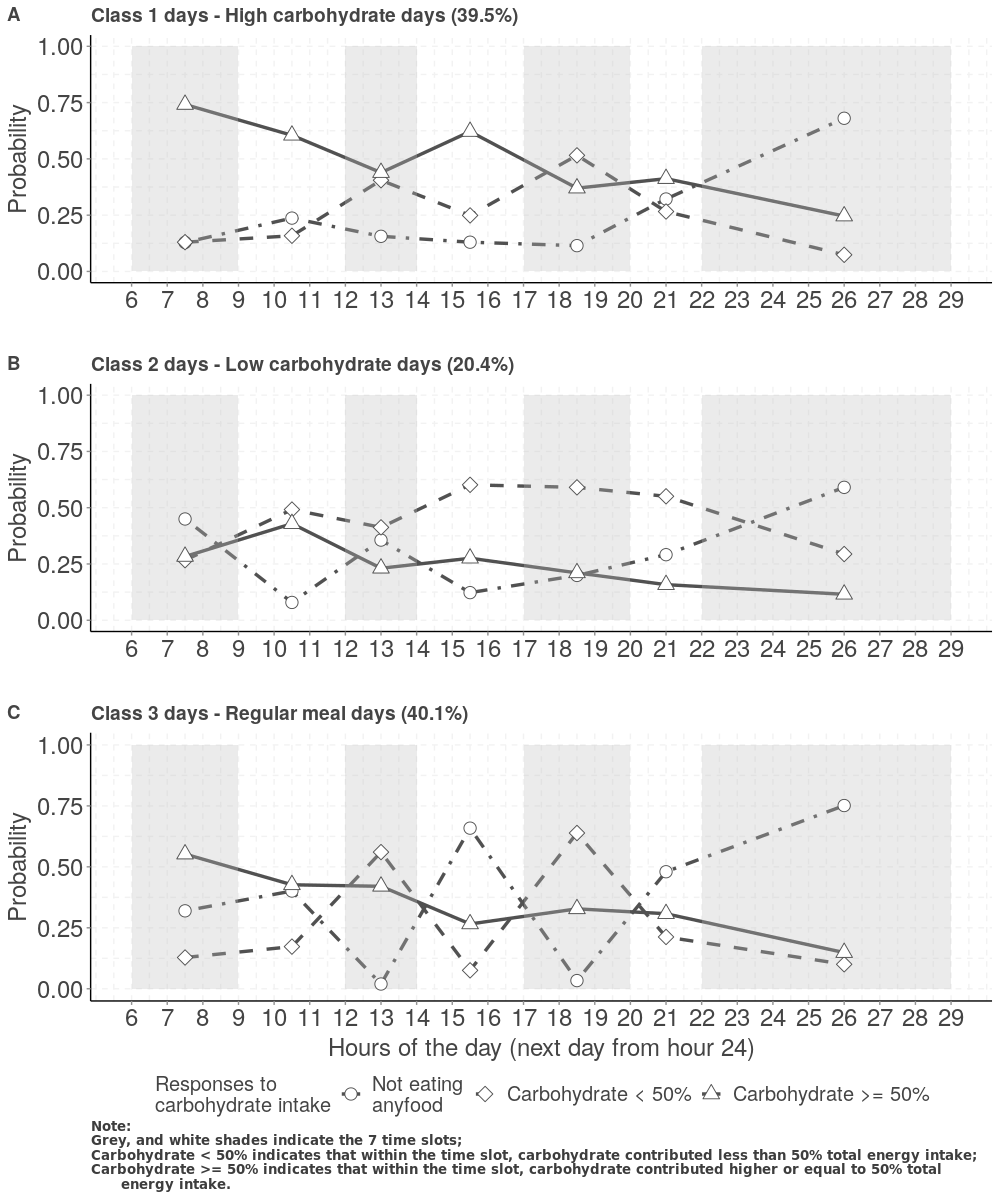
\includegraphics[width=13cm]{Figures/level1.png}
	\decoRule
	\caption[Day Level Latent Class Solution.]{Day Level Latent Classes Solution.}
	\label{fig:level1}
\end{figure}
\vspace{-0.6cm}

Class 3 days \textbf{(Figure \ref{fig:level1}-C)} were called "regular meals day" due to the following reasons: 1) participants' dietary recordings showed that in these days there was almost 0 possibility of not eating any food at lunch (0.019 between 12 noon and 2 pm) and dinner (0.034 between 5 pm and 8 pm); 2) the probabilities of not eating during morning snack time (9 am to 12 noon) and afternoon snack time (2 pm to 5 pm) were also the highest among the three types of days (0.401 and 0.659). 3) during these days, participants may have some high carbohydrate contained food between 8 pm and 10 pm (probability = 0.308), but the probability of not eating any food during 10 pm to 6 am next morning was 0.751, the highest among the three types of days. \vspace{-0.5cm}


\subsection{Features of the three types of carbohydrate eating temporal patterns}

\rowcolors{2}{gray!6}{white}

\begin{table}
	
	\caption{\label{tab:day-level-features}Means (standard deviations), and counts (\%) of the characteristics of different types of carbohydrate eating days.}\vspace{-0.3cm}
	\centering
	\fontsize{9}{11}\selectfont
	\begin{tabular}[t]{lcccc}
		\hiderowcolors
		\toprule
		& \textbf{\Centerstack{High perc-\\entage carb}} & \textbf{\Centerstack{Low perc-\\entage carb}} & \textbf{\Centerstack{Regular\\meals}} & \textbf{\textit{P} value}\textsuperscript{*}\\
		\midrule
		\showrowcolors
		Counts (\%) & 9667 (39.5) & 5002 (20.4) & 9814 (40.1) & \\
		Country (\%) &  &  &  & < 0.001\\
		\hspace{1em}England & 5627 (58.2) & 2972 (59.4) & 5291 (53.9) & \\
		\hspace{1em}Northern Ireland & 1194 (12.4) & 527 (10.5) & 1400 (14.3) & \\
		\hspace{1em}Scotland & 1527 (15.8) & 813 (16.3) & 1774 (18.1) & \\
		\hspace{1em}Wales & 1318 (13.6) & 690 (13.8) & 1349 (13.7) & \\
		Day of Week (\%) &  &  &  & < 0.001\\
		\hspace{1em}Monday & 1303 (13.5) & 715 (14.3) & 1370 (14.0) & \\
		\hspace{1em}Tuesday & 1266 (13.1) & 674 (13.5) & 1290 (13.1) & \\
		\hspace{1em}Wednesday & 1225 (12.7) & 740 (14.8) & 1233 (12.6) & \\
		\hspace{1em}Thursday & 1272 (13.2) & 752 (15.0) & 1425 (14.5) & \\
		\hspace{1em}Friday & 1458 (15.1) & 797 (15.9) & 1479 (15.1) & \\
		\hspace{1em}Saturday & 1537 (15.9) & 703 (14.1) & 1495 (15.2) & \\
		\hspace{1em}Sunday & 1605 (16.6) & 621 (12.4) & 1522 (15.5) & \\
		\hspace{1em}Weekend, Yes (\%) & 3142 (32.5) & 1324 (26.5) & 3017 (30.7) & < 0.001\\
		Total energy (kJ) & 7539.98 (2875.87) & 7160.22 (2922.15) & 7439.68 (2978.91) & < 0.001\\
		Carbohydrate (g) & 222.79 (89.84) & 209.70 (86.17) & 206.59 (84.42) & < 0.001\\
		Protein (g) & 71.36 (29.79) & 69.55 (30.20) & 73.29 (32.94) & < 0.001\\
		Fat (g) & 65.44 (33.27) & 63.94 (33.76) & 67.24 (34.73) & < 0.001\\
		Alcohol (g) & 11.76 (27.31) & 8.85 (24.25) & 13.80 (33.00) & < 0.001\\
		Total sugars (g) & 98.63 (56.03) & 88.03 (50.50) & 86.39 (50.96) & < 0.001\\
		Starch (g) & 124.07 (55.84) & 121.59 (56.13) & 120.11 (54.62) & < 0.001\\
		Non-milk extrinsic sugar\textsuperscript{\dag} & 59.45 (49.31) & 50.07 (43.41) & 50.41 (44.84) & < 0.001\\
		Fruit (g) & 107.40 (137.97) & 103.15 (129.08) & 92.76 (126.02) & < 0.001\\
		Yellow Red Green Vegetables (g) & 26.52 (46.44) & 26.84 (47.99) & 26.16 (45.99) & 0.681\\
		\bottomrule
		\multicolumn{5}{l}{{\scriptsize \textit{Note:} carb is short for carbohydrate.}}\\
		\multicolumn{5}{l}{{\scriptsize \textsuperscript{*} \textit{P} values were obtained from Pearson $\chi^2$ test for categorical variables, and one-way ANOVA comparing the means}}\\
		\multicolumn{5}{l}{{\scriptsize  in multiple groups for continuous variables;}}\\
		\multicolumn{5}{l}{{\scriptsize \textsuperscript{\dag} Non-milk extrinsic sugar is defined as: additionally added free sugar, such as table sugar, honey, glucose, fructose}}\\ 
		\multicolumn{5}{l}{{\scriptsize and glucose syrups, sugars added to food and sugars in fruit juices.}}\\
	\end{tabular}
\end{table}

\rowcolors{2}{white}{white}
\vspace{-0.5cm}

The details of the characteristics of the three types of carbohydrate eating time pattern were listed in\textbf{ Table \ref{tab:day-level-features}}. Specifically, regular meals day turned to be recorded slightly more often in Northern Ireland, and Scotland. In terms of day of week distribution in the three types of days, there is strong evidence (\textit{p} < 0.001) that high carbohydrate days appeared more frequently in weekends (32.5\%) compared with low carbohydrate day (26.5\%) and regular meals day (30.7\%).

As expected, consumption of total energy (7539.98 kJ), total carbohydrate (222.79 g), total sugar (98.63 g), starch (124.07 g), and non-milk extrinsic sugar (59.45 g) were the highest among high percentage carbohydrate days (all \textit{p} < 0.001). On the other hand, the consumption of protein (73.29 g), total fat (67.24 g), and alcohol (13.80 g) were the highest in the regular meals days. Moreover, in high percentage carbohydrate days, participants turned to consume the highest amount of fruit (107.40 g). There was no evidence of any difference for the consumption of yellow, red, or green vegetables across the three types of days (\textit{p} = 0.681).\vspace{-0.6cm}

%---------------------------------
%	SUBSECTION 2
%-----------------------------------

\subsection{Individual level LCA solution}\vspace{-0.3cm}

In the random effect models we utilized the non-parametric approach, in which we added a level 2 (individual level) latent classes based on the random means from the level 1 (day level) latent class solution. The results of the individual level LCA solution for 2 and 3 classes are presented in \textbf{Figure \ref{fig:CB2level2}}, and \textbf{\ref{fig:level2}}. 


\begin{figure}[H]
	%\vspace*{13cm}
	\centering
	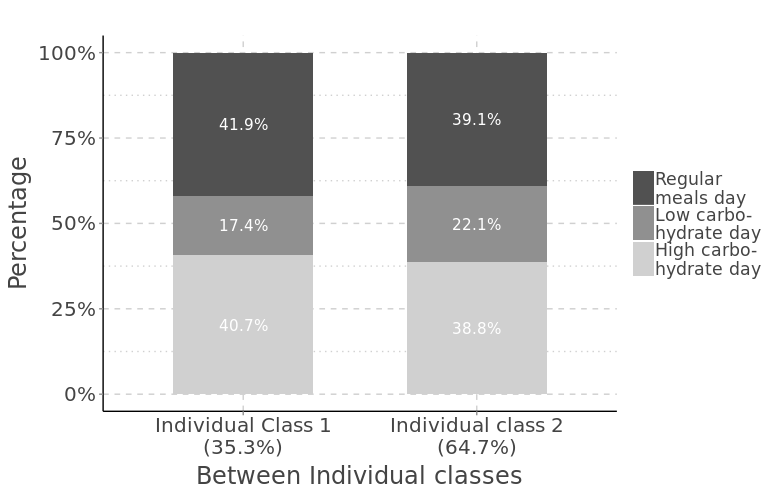
\includegraphics[width=11cm]{Figures/CB2level2.png}
	\decoRule
	\caption[Multilevel Latent Class Solution ($3\times2$).]{Multilevel Latent Class Solution, 3 classes in day level, 2 classes in individual level.}
	\label{fig:CB2level2}
\end{figure}

With two individual level latent classes \textbf{(Figure \ref{fig:CB2level2})}, one individual class is comprised of individuals with a relatively slightly higher proportion of having "low carbohydrate day" (22.1\%) compared to the other (17.4\%). This class represents nearly 65\% of the individuals. However, we believe these individual classes are not very distinguishable to each other.

With three individual level latent classes \textbf{(Figure \ref{fig:level2})}, a low-carbohydrate eaters class, a moderate-carbohydrate eaters class, and a high-carbohydrate eaters class emerges. 43.1\% participants were identified as high-carbohydrate eaters, in these individuals, about 50\% of the days (2 out of 4 days) of their dietary diary could be classified as having high carbohydrate days. Nearly 1 out of 4 days of their dietary diary were either "regular meals day" or "low carbohydrate day". 28.1\% participants fell into the low carbohydrate eaters class in the left hand side of \textbf{Figure \ref{fig:level2}}, their recordings of food intake showed that in more than 60\% of their days, they were having "regular meals" which was characterised as with highest amount of fat and alcohol consumptions as already described in \textbf{Table \ref{tab:day-level-features}}. Moderate carbohydrate eaters have comparable proportions (42.0\% vs. 40.0\%) of having high carbohydrate days and regular meals day, 18.0\% of their dietary diary were found to be low carbohydrate days.

\begin{figure}
	%\vspace*{13cm}
	\centering
	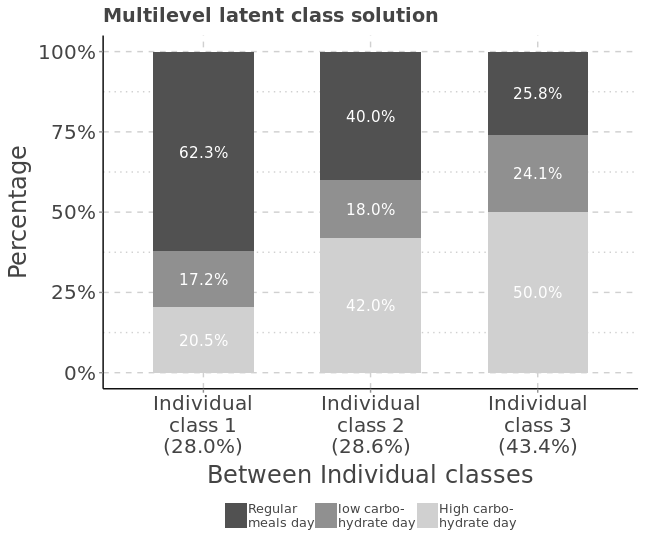
\includegraphics[width=11cm]{Figures/level2.png}
	\decoRule
	\caption[Multilevel Latent Class Solution ($3\times3$).]{Multilevel Latent Class Solution, 3 classes in day level, 3 classes in individual level.}
	\label{fig:level2}
\end{figure}

After recognising that there were three potential latent groups of carbohydrate eaters in the UK adults, whose food consumption pattern were also probably switching from one to another during the survey, their average carbohydrate contribution to total energy intake (as well as the subtypes of carbohydrate actually consumed) within the 7 pre-defined time slots of the day were still of interest. Survey-design-weighted mean energy intake within each time slot of the day and their composition of contribution are illustrated in \textbf{Figure \ref{fig:energysourcesCB}}, weighted mean nutrients intakes are listed in \textbf{Table \ref{tab:tab-nutri-indi}}.

\begin{figure}[H]
	%\vspace*{13cm}
	\centering
	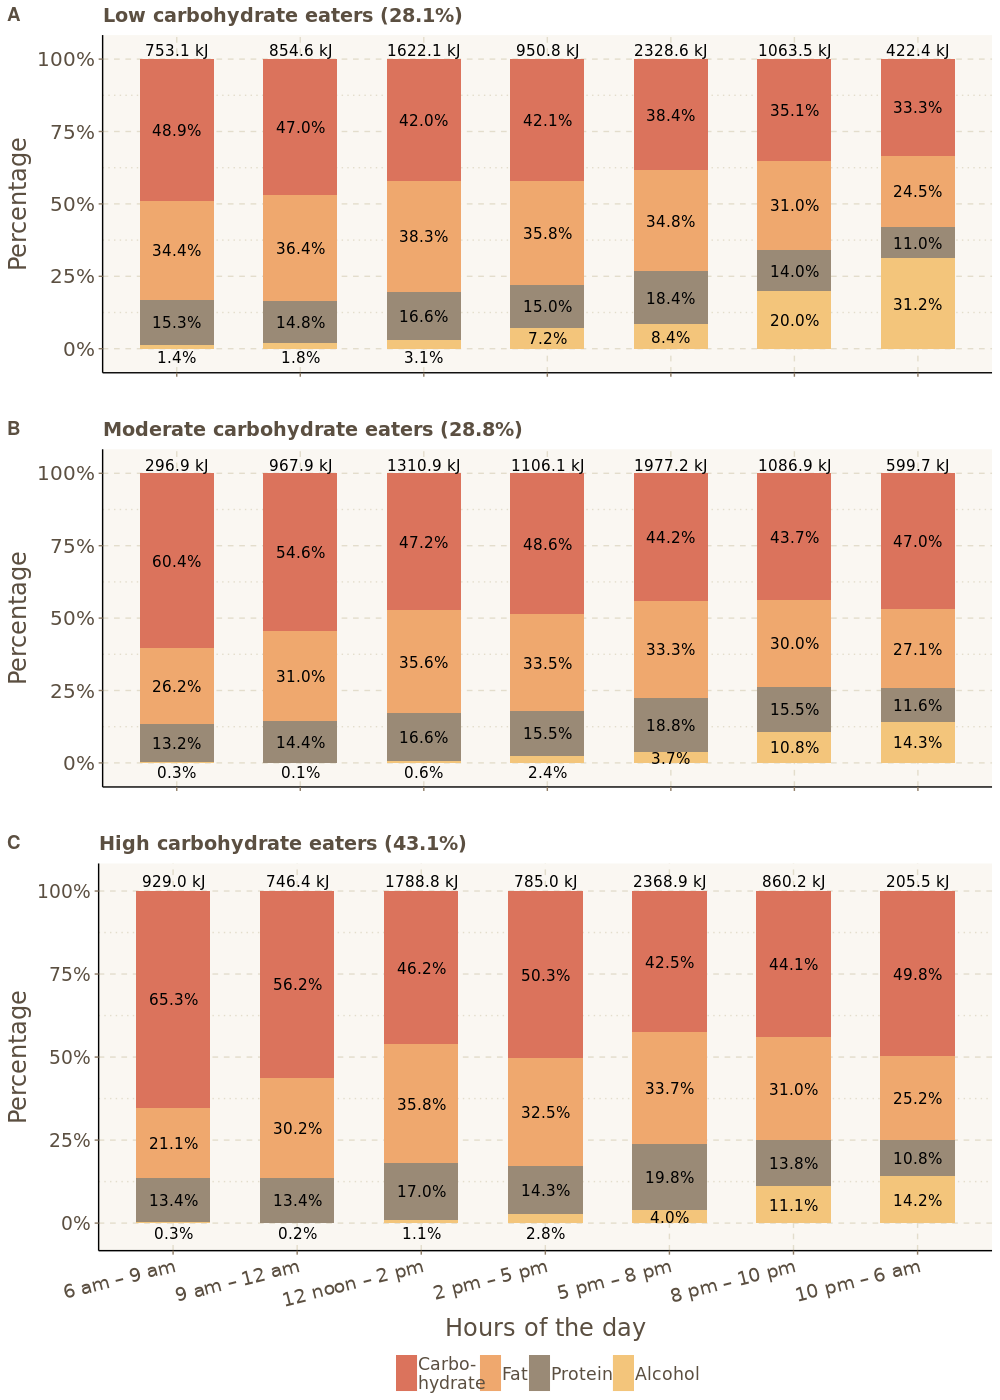
\includegraphics[width=13cm]{Figures/CBenergysources.png}
	\decoRule
	\caption[Sources of Energy Contribution at Each Time Slot by Individual Carbohydrate Eating Groups.]{Sources of Energy Contribution at Each Time Slot by Individual Carbohydrate Eating Groups.}
	\label{fig:energysourcesCB}
\end{figure}
\vspace{-0.6cm}

Among the three types of carbohydrate eaters, the mean of total energy intake over the 4 days of dietary survey was the highest (7985.8 kJ, 95\%CI: 7283.3, 8146.3) in the low carbohydrate eaters group, and the lowest (7341.8 kJ, 95\%CI: 7172.5, 7511.2) in the moderate eaters group \textbf{(Table \ref{tab:tab-nutri-indi})}. Sources of energy for each type of carbohydrate eaters by the 7 time slots were also different. Low carbohydrate eaters \textbf{(Figure \ref{fig:energysourcesCB}-A)} never had carbohydrate contributed more than 50\% of their total energy throughout the day. Energy from fat were the highest for low carbohydrate eaters most of the time during the day (except for time between 10 pm to 6 am next morning). Most impressively, energy from alcohol were always the highest in low carbohydrate eaters, percentages for energy from alcohol for the 7 times slots were 1.4\% (6-9 am), 1.8\% (9-12 noon), 3.1\% (12-2 pm), 7.2\% (2-5 pm), 8.4\% (5-8 pm), 20.0\% (8-10 pm), and 31.2\% (10 - 6 am), respectively. Contribution from different energy sources are quite similar for moderate and high carbohydrate eaters, but their absolute amount of energy consumption at each time slot were largely different. Moderate carbohydrate eaters \textbf{(Figure \ref{fig:energysourcesCB}-B)} were characterised as consuming the lowest energy (296.9 kJ) before 9 am, but having higher energy consumption (967.9 kJ) between 9 am and 12 noon time compared with low and high carbohydrate eaters. Moderate carbohydrate eaters may turn to have later breakfast, later lunch, and probably later dinner as well. They had the highest total energy consumption (599.7 kJ) at night (10 pm - 6 am) across three types of eaters. High carbohydrate eaters \textbf{(Figure \ref{fig:energysourcesCB}-C)} consumed the highest total energy (929.0 kJ) during 6 am to 9 am in the morning and the lowest total energy between 10 pm to 6 am (205.5 kJ). Specifically, carbohydrate contribution to total energy intake were 65.3\% (6-9 am), 56.2\% (9-12 noon), 46.2\% (12-2 pm), 50.3\% (2-5 pm), 42.5\% (5-8 pm), 44.1\% (8-10 pm), and 49.9\% (10-6am). We also noticed that high carbohydrate eaters consumed their energy mainly from three time slots: 6-9 am, 12-2 pm, and 5-8 pm. 

As expected, in total, the mean of carbohydrate intake was 203.8 g, 218.3 g, and 233.4 g for low, moderate, and high carbohydrate eaters, respectively \textbf{(Table \ref{tab:tab-nutri-indi})}. Energy contribution from carbohydrate was close to 50\% in the high carbohydrate eaters, but was only 40.6\% in the low carbohydrate eaters. In terms of the subtypes (components) of the carbohydrate consumed at each time slot, high carbohydrate eaters consumed as much as more than 2 times (compared to low carbohydrate eaters) and nearly 4 times (against moderate carbohydrate eaterss) the amount of sugar (37.9g 95\% CI: 36.8, 39.2) and non-milk extrinsic sugar (i.e. free sugar) (11.1g 95\%CI: 10.7, 11.6) between 6-9 am. Moderate carbohydrate eaters had their carbohydrate intake more spread out. They consumed more sugar and starch during 9-12 noon, 2-5 pm, 8-10 pm, and 10-6 am. Low carbohydrate eaters turned to have similar temporal pattern of consuming carbohydrates but the absolute amount of fibre, sugar, free sugar, and starch were usually lower than that in the high carbohydrate eaters except for time slots of 2-5 pm, and 10-6 am. Strong evidence (\textit{p} < 0.001) suggested that the mean of total fibre consumption for low,




\rowcolors{2}{gray!6}{white}

\begin{table}[H]
	
	\caption{\label{tab:tab-nutri-indi}Weighted means and percentages (95\%CI) of the nutrients intake according to individual level carbohydrate eating classes.  \\ (NDNS RP 2008/09-15/16, sample size = 6155)}\vspace{-0.3cm}
	\centering
	\fontsize{9}{11}\selectfont
	\begin{tabular}[t]{lcccc}
		\hiderowcolors
		\toprule
	\textbf{Variables} & \textbf{\Centerstack{Low carbo-\\hydrate eaters\\(n = 1730)}} & \textbf{\Centerstack{Moderate carbo-\\hydrate eaters\\(n = 1772)}} & \textbf{\Centerstack{High carbo-\\hydrate eaters\\(n = 2653)}} & \textbf{\textit{P} value} \textsuperscript{*}\\
		\midrule
		\showrowcolors
		Total energy (kJ) & 7985.8 (7823.3, 8146.3) & 7341.8 (7172.5, 7511.2) & 7677.8 (7555.8, 7799.8) & < 0.001\\
		Carbohydrate (g) & 203.8 (199.8, 207.8) & 218.3 (212.9, 223.7) & 233.4 (229.6, 237.2) & < 0.001\\
		\hspace{1em}\textbf{6 am – 9 am} & 23.0 (21.8,  24.3) & 11.2 (10.0, 12.3) & 37.9 (36.8, 39.2) & \\
		\hspace{2em}Fibre (g) & 1.4 (1.3, 1.5) & 0.6 (0.5, 0.7) & 2.0 (1.9, 2.2) & \\
		\hspace{2em}Sugar (g) & 10.2 (9.6, 10.9) & 5.3 (4.8, 5.8) & 19.7 (19.0, 20.4) & \\
		\hspace{3em}NMES (g)\textsuperscript{\dag} & 4.7 (4.3, 5.1) & 3.2 (2.9, 3.6) & 11.1 (10.7, 11.6) & \\
		\hspace{2em}Starch (g) & 12.8 (12.0, 13.5) & 5.9 (5.1, 6.6) & 18.3 (17.6, 19.1) & \\
		\hspace{1em}\textbf{9 am – 12 noon} & 25.1 (23.9, 26.3) & 33.0 (31.4, 34.6) & 26.2 (25.1, 27.2) & \\
		\hspace{2em}Fibre (g) & 1.5 (1.4, 1.6) & 1.6 (1.5, 1.7) & 1.3 (1.2, 1.3) & \\
		\hspace{2em}Sugar (g) & 11.6 (10.9, 12.3) & 15.7 (14.8, 16.6) & 14.2 (13.6, 14.8) & \\
		\hspace{3em}NMES (g)\textsuperscript{\dag} & 5.7 (5.2, 6.2) & 9.6 (8.9, 10.2) & 8.1 (7.7, 8.5) & \\
		\hspace{2em}Starch (g) & 13.5 (12.8, 14.3) & 17.3 (16.4, 18.3) & 11.9 (11.3, 12.6) & \\
		\hspace{1em}\textbf{12 noon – 2 pm} & 42.6 (40.9, 44.3) & 38.7 (37.0, 40.4) & 51.6 (50.2, 52.9) & \\
		\hspace{2em}Fibre (g) & 3.1 (2.9, 3.2) & 2.3 (2.2, 2.5) & 3.6 (3.5, 3.7) & \\
		\hspace{2em}Sugar (g) & 14.7 (14.0, 15.4) & 14.9 (14.0, 15.7) & 19.4 (18.7, 20.0) & \\
		\hspace{3em}NMES (g)\textsuperscript{\dag} & 7.3 (6.7, 7.8) & 9.1 (8.4, 9.8) & 10.3 (9.8, 10.8) & \\
		\hspace{2em}Starch (g) & 27.9 (26.6, 29.1) & 23,8 (22.6, 24.9) & 32.2 (31.2, 33.1) & \\
		\hspace{1em}\textbf{2 pm – 5 pm} & 25.0 (23.6, 26.4) & 33.6 (31.6, 35.6) & 24.7 (23.6, 25.7) & \\
		\hspace{2em}Fibre (g) & 1.6 (1.5, 1.7) & 1.9 (1.7, 2.0) & 1.3 (1.2, 1.4) & \\
		\hspace{2em}Sugar (g) & 11.9 (11.3, 12.7) & 14.5 (13.5, 15.5) & 13.4 (12.8, 13.9) & \\
		\hspace{3em}NMES (g)\textsuperscript{\dag} & 6.9 (6.4, 7.5) & 9.9 (9.0, 8.6) & 8.6 (8.2, 9.1) & \\
		\hspace{2em}Starch (g) & 13.1 (12.1, 13.9) & 19.1 (17.7, 20.4) & 11.3 (10.6, 11.9) & \\
		\hspace{1em}\textbf{5 pm – 8 pm} & 55.9 (54.1, 57.9) & 54.6 (52.1, 57.0) & 62.9 (61.3, 64.4) & \\
		\hspace{2em}Fibre (g) & 4.4 (4.2, 4.5) & 3.7 (3.5, 3.9) & 4.9 (4.7, 5.0) & \\
		\hspace{2em}Sugar (g) & 18.7 (17.9, 19.5) & 18.6 (17.6, 19.5) & 21.8 (20.9, 22.5) & \\
		\hspace{3em}NMES (g)\textsuperscript{\dag} & 10.2 (9.6, 10.8) & 11.8 (10.9, 12.6) & 12.1 (11.4, 12.7) & \\
		\hspace{2em}Starch (g) & 37.3 (35.8, 38.8) & 35.9 (34.1, 37.9) & 41.1 (39.9, 42.2) & \\
		\hspace{1em}\textbf{8 pm – 10 pm} & 23.3 (21.9, 24.6) & 29.7 (27.6, 31.7) & 23.7 (22.5, 24.9) & \\
		\hspace{2em}Fibre (g) & 1.4 (1.3, 1.6) & 1.6 (1.5, 1.8) & 1.3 (1.5, 1.8) & \\
		\hspace{2em}Sugar (g) & 10.9 (10.3, 11.5) & 13.2 (12.2, 14.2) & 12.4 (11.8, 13.0) & \\
		\hspace{3em}NMES (g)\textsuperscript{\dag} & 7.3 (6.8, 7.8) & 9.4 (8.5, 10.4) & 8.3 (7.8, 8.8) & \\
		\hspace{2em}Starch (g) & 12.3 (11.4, 13.3) & 16.4 (15.0, 17.8) & 11.3 (10.5, 12.1) & \\
		\hspace{1em}\textbf{10 pm – 6 am} & 8.8 (7.7, 9.8) & 17.6 (15.2, 19.9) & 6.4 (5.8, 7.1) & \\
		\hspace{2em}Fibre (g) & 0.34 (0.29, 0.39) & 0.74 (0.63, 0.85) & 0.24 (0.21, 0.27) & \\
		\hspace{2em}Sugar (g) & 5.3 (4.6, 6.1) & 10.0 (8.6, 11.5) & 4.1 (3.7, 4.5) & \\
		\hspace{3em}NMES (g)\textsuperscript{\dag} & 3.9 (3.3, 4.6) & 7.7 (6.4, 8.9) & 2.9 (2.6, 3.3) & \\
		\hspace{2em}Starch (g) & 3.5 (2.9, 3.9) & 7.5 (6.3, 8.8) & 2.3 (1.9, 2.7) & \\
		Carbohydrate (\%) & 40.6 (40.2, 41.0) & 47.3 (46.8, 47.8) & 48.3 (47.9, 48.6) & < 0.001\\
		Fibre (g) & 13.7 (13.4, 14.0) & 12.5 (12.1, 12.9) & 14.7 (14.4, 14.9) & < 0.001 \\
		Protein (g) & 79.9 (77.9, 81.8) & 69.3 (67.6, 71.0) & 73.7 (72.5, 74.8) & < 0.001\\
%		Protein (\%) & 17.2 (16.9, 17.5) & 16.3 (16.0, 16.6) & 16.5 (16.3, 16.6) & < 0.001\\
		Fat (g) & 74.7 (73.1, 76.4) & 63.8 (62.1, 65.5) & 65.7 (64.4, 67.0) & < 0.001\\
%		Fat (\%) & 35.4 (34.9, 35.8) & 32.5 (32.1, 32.9) & 32.0 (31.7, 32.3) & < 0.001\\
		Alcohol (g) & 20.8 (18.3, 23.2) & 10.7 (9.4, 11.9) & 8.9 (8.1, 9.8) & < 0.001\\
		\bottomrule
		\multicolumn{5}{l}{{\scriptsize \textsuperscript{*} \textit{P} values were obtained from $\chi^2$ test for categorical variables, and one-way ANOVA comparing the means}}\\
		\multicolumn{5}{l}{{\scriptsize  in multiple groups for continuous variables;}}\\
		\multicolumn{5}{l}{\textsuperscript{\dag} NMES, Non-milk extrinsic sugar is defined as: additionally added free sugar, such as table sugar, honey, }\\
		\multicolumn{5}{l}{{\scriptsize glucose, fructose and glucose syrups, sugars added to food and sugars in fruit juices.}}\\
	\end{tabular}
\end{table}

\rowcolors{2}{white}{white}

moderate, and high carbohydrate eaters were different: 13.7g (13.4, 14.0), 12.5g (12.1, 12.9), and 14.7g (14.4, 14.9) with all 95\% CI being exclusive to each other. It is also noteworthy that low carbohydrate eaters consumed the highest average amount of protein (79.9 g, 17.2\% of total energy), fat (74.7g, 35.4\% of total energy), and alcohol (20.8 g, 6.8\% of total energy) as we have described for \textbf{Figure \ref{fig:energysourcesCB}}. 
 
The social-demographic characteristics of the UK adults according to their individual level latent class membership are shown in \textbf{Table \ref{tab:Level2tab1}}. Moderate carbohydrate eaters were relatively younger (\textit{p} < 0.001), and slightly less from England (\textit{p} = 0.007). Gender distribution across the three types of carbohydrate eaters was fairly even (\textit{p} = 0.119). The distribution of the carbohydrate eater types turned out to be changing with the year of survey. Low carbohydrate eaters represented 32.5\% of the population in the first year of survey, but later dropped to lower than 30\% (lowest in the third year, 22.6\%) until the most recent year. Proportion of high carbohydrate eaters increased from 41.2\% to the highest (50.6\%) in the second year, but then started to decline to 38.4\% in the 8th year of survey (\textit{p} = 0.015). There was no evidence of difference in employment status across three types of carbohydrate eaters. However, strong evidence suggested that high carbohydrate eaters had the highest proportion (61.3\%) of living with partner (\textit{p} < 0.001); moderate carbohydrate eaters had the lowest average income (27180.8 \textsterling/year), highest proportion of non-white population (20.5\%), and lower education level (23.3\% with degree of higher education) compared with either low or high carbohydrate eaters. 


Weighted means, percentages of anthropometric measurements, average of main nutrients intake, as well as biochemical characteristic profiles according to the latent carbohydrate eater groups are given in \textbf{Table \ref{tab:tab2}}. Low carbohydrate eaters had higher mean BMI (27.8 kg/m\textsuperscript{2}) and larger mean WC (98.9/89.9 cm in men/women) compared with 27.2, 27.3 kg/m\textsuperscript{2}, and 95.9/88.7 (men/women), 98.1/87.2 (men/women) cm in moderate and high carbohydrate eaters. Moderate carbohydrate eaters had the highest prevalence of being a current smoker (27.8\%), shortest time of daily physical activity (geometric mean: 0.87 hours/day), and the lowest prevalence of hypertension (20.2\%).

From the results of blood tests, 6.9\% of low carbohydrate eaters were found to be diabetic (diagnosed by A1C > 6.5\%), while the percentages of diabetes in the moderate and high carbohydrate eaters were 3.5\%, and 4.1\% (\textit{p} < 0.011), respectively. Although there was some evidence (\textit{p} = 0.027) that fasting blood glucose level may be slightly higher in non-diabetic low carbohydrate eaters, the geometric mean for


\rowcolors{2}{gray!6}{white} 

\begin{table}[H]

\caption{\label{tab:Level2tab1}Weighted means, percentages, and
95\% CIs of the social-demographic characteristics by carbohydrate eating latent class memberships in the UK
adults. \\ (NDNS RP 2008/09-15/16, sample size = 6155)} \centering
\fontsize{9}{11}\selectfont

\begin{tabular}[t]{lcccc}
	\hiderowcolors
	\toprule
	\textbf{Variables} & \textbf{\Centerstack{Low carbo-\\hydrate eaters\\(n = 1730)}} & \textbf{\Centerstack{Moderate carbo-\\hydrate eaters\\(n = 1772)}} & \textbf{\Centerstack{High carbo-\\hydrate eaters\\(n = 2653)}} & \textbf{\textit{P} value} \textsuperscript{*}\\
	\midrule
	\showrowcolors
	Total (\%) & 28.4 (26.9, 29.9) & 28.7 (27.1, 30.3) & 43.0 (41.3, 44.7) & \\
	Country (\%) &  &  &  & 0.007\\
	\hspace{1em}England & 84.5 (81.7, 86.9) & 82.0 (79.3, 84.5) & 84.7 (82.3, 86.8) & \\
	\hspace{1em}Northern Ireland & 2.1 (1.6, 2.8) & 4.2 (3.2, 5.6) & 2.2 (1.7, 3.0) & \\
	\hspace{1em}Scotland & 9.1 (7.0, 11.8) & 8.6 (6.7, 11.1) & 8.0 (6.3, 10.2) & \\
	\hspace{1em}Wales & 4.3 (3.3, 5.6) & 5.1 (4.0, 6.4) & 5.1 (4.0, 6.4) & \\
	Age (years) & 51.0 (49.9, 52.1) & 40.3 (39.1, 41.6) & 51.7 (50.7, 52.7) & < 0.001\\
	Sex (\%) &  &  &  & 0.119\\
	\hspace{1em}Men & 50.0 (46.9, 53.1) & 50.2 (47.0, 53.5) & 46.6 (44.0, 49.1) & \\
	\hspace{1em}Women & 50.0 (46.9, 53.1) & 49.8 (46.5, 53.0) & 53.4 (50.9, 56.0) & \\
	Survey years (\% in rows) &  &  &  & 0.015\\
	\hspace{1em}1 & 32.5 (28.4, 36.9) & 26.3 (21.9, 31.2) & 41.2 (36.6, 46.0) & \\
	\hspace{1em}2 & 26.8 (22.6, 31.3) & 22.6 (18.6, 27.3) & 50.6 (45.8, 55.4) & \\
	\hspace{1em}3 & 22.6 (18.8, 26.9) & 33.7 (28.6, 39.2) & 43.6 (38.7, 48.7) & \\
	\hspace{1em}4 & 27.9 (24.1, 32.2) & 27.6 (23.8, 31.8) & 44.4 (40.2, 48.7) & \\
	\hspace{1em}5 & 27.9 (24.2, 32.0) & 28.7 (24.4, 33.5) & 43.3 (38.2, 48.6) & \\
	\hspace{1em}6 & 28.0 (24.0, 32.4) & 31.5 (26.9, 36.6) & 40.5 (35.8, 45.3) & \\
	\hspace{1em}7 & 29.1 (25.2, 33.4) & 29.0 (24.5, 34.0) & 41.8 (37.1, 46.7) & \\
	\hspace{1em}8 & 31.1 (27.3, 35.3) & 30.5 (25.9, 35.5) & 38.4 (34.1, 42.8) & \\
	Paid employment\textsuperscript{\dag} (\%) &  &  &  & 0.907\\
	\hspace{1em}Yes & 40.3 (37.0, 43.6) & 40.8 (37.1, 44.5) & 39.8 (37.1, 42.6) & \\
	\hspace{1em}No & 59.7 (56.4, 63.0) & 59.2 (55.5, 62.9) & 60.2 (57.4, 62.9) & \\
	Live with partner\textsuperscript{\ddag} (\%) &  &  &  & < 0.001\\
	\hspace{1em}Yes & 56.9 (53.6, 60.1) & 38.4 (35.2, 41.8) & 61.3 (58.7, 63.7) & \\
	\hspace{1em}No & 43.1 (39.9, 46.4) & 61.6 (58.2, 64.8)) & 38.7 (36.3, 41,3) & \\
	Household income, \textsterling/year & \Centerstack{36558.5\\(34800.2, 38316.8)} & \Centerstack{27180.8\\(25597.9, 28763.7)} & \Centerstack{32171.6\\(31024.9, 33318.2)} & < 0.001\\
	Ethnicity (\%) &  &  &  & \\
	\hspace{1em}White & 94.2 (92.4, 95.6) & 79.5 (76.4, 82.3) & 91.9 (90.1, 93.4) & < 0.001\\
	\hspace{1em}Non-White & 5.8 (4.4, 7.6) & 20.5 (17.7, 23.6) & 8.1 (6.6, 9.9) & \\
	Education (\%) &  &  &  & \\
	\hspace{1em}Degree or higher & 29.0 (26.1, 32.1) & 23.3 (20.5, 26.3) & 26.2 (24.1, 28.5) & 0.019\\
	\hspace{1em}Lower than degree & 71.0 (67.9, 73.9) & 76.7 (73.7, 79.5) & 73.8 (71.5, 75.9) & \\
	\bottomrule
	\multicolumn{5}{l}{{\scriptsize \textit{Note: }}}\\
	\multicolumn{5}{l}{{\scriptsize \textbf{Abbreviations}: CI, confidence intervals; NDNS RP, national diet and nutrition survey rolling programme.}}\\
	\multicolumn{5}{l}{{\scriptsize Variables were weighted by individual weights.}}\\
	\multicolumn{5}{l}{{\scriptsize \textsuperscript{*} For continuous variables, the \textit{F} test was used to determine differences between latent classes with Bonferroni}}\\ 
	\multicolumn{5}{l}{{\scriptsize correction to account for multiple testing across $>$ 2 classes. For categorical variables, differences between}}\\
	\multicolumn{5}{l}{{\scriptsize  latent classes were assessed using the adjusted Pearson $\chi^2$ test for survey data.}} \\
	\multicolumn{5}{l}{{\scriptsize \textsuperscript{\dag} Paid employment was defined as being in paid employment during the last 4 weeks prior to the survey.} }\\
	\multicolumn{5}{l}{{\scriptsize \textsuperscript{\ddag} Live with partner was defined as either living with a married husband/wife or a legally recognised civil}} \\
	\multicolumn{5}{l}{{\scriptsize partnership.}}\\
\end{tabular}

\end{table} 
\rowcolors{2}{white}{white}

A1C was probably lower in moderate carbohydrate eaters (4.72, 95\%CI: 5.39, 5.47). Total cholesterol, HDL, and LDL were all lower in the moderate carbohydrate eaters, while no evidence of any difference of TG was found across three types of carbohydrate eaters. 




\rowcolors{2}{gray!6}{white}

\begin{table}[H]
	
	\caption{\label{tab:tab2}Weighted means, percentages, and 95\% CIs of the anthropometric measurements, average main nutrients intake and biochemical characteristics by carbohydrate eating latent class memberships in the UK adults. (NDNS RP 2008/09-15/16, sample size = 6155)}
	\centering
	\fontsize{9}{11}\selectfont
	\begin{tabular}[t]{lcccc}
		\hiderowcolors
		\toprule
	\textbf{Variables} & \textbf{\Centerstack{Low carbo-\\hydrate eaters\\(n = 1730)}} & \textbf{\Centerstack{Moderate carbo-\\hydrate eaters\\(n = 1772)}} & \textbf{\Centerstack{High carbo-\\hydrate eaters\\(n = 2653)}} & \textbf{\textit{P} value} \textsuperscript{*}\\
		\midrule
		\showrowcolors
		BMI (kg/m\textsuperscript{2}) & 27.8 (27.4, 28.2) & 27.2 (26.7, 27.7) & 27.3 (26.9, 27.6) & 0.006\\
		WC (cm) &&&& \\ 
		\hspace{1em}Men &  98.9 (97.4, 100.5) & 95.9 (94.1, 97.8) &  98.1 (96.9, 99.2) & 0.056\\
		\hspace{1em}Women & 89.9 (88.7, 91.3) &  88.7 (87.1, 90.3) &  87.2 (86.1, 88.2) & 0.005\\
		Smoking status (\%) &  &  &  & \\
		\hspace{1em}Current & 20.4 (18.0, 23.0) & 27.8 (25.0, 30.9) & 17.1 (15.4, 19.0) & < 0.001\\
		\hspace{1em}Ex-smoker & 29.3 (26.5, 32.2) & 16.8 (14.6, 19.2) & 26.1 (24.9, 28.3) & \\
		\hspace{1em}Never & 50.3 (47.2, 32.2) & 55.4 (52.2, 58.6) & 56.8 (54.3, 59.3) & \\
		Physical activity (hours/day) \textsuperscript{\P} & 1.08 (0.97, 1.19) & 0.87 (0.77, 0.97)  & 1.07 (0.98, 1.16) & 0.005 \\
		Hypertension\textsuperscript{\dag}, Yes (\%) & 33.8 (30.2, 37.5) & 20.2 (17.0, 24.0) & 30.9 (26.9, 31.0) & < 0.001\\
		Total energy intake (kJ) & \Centerstack{7985.8\\(7823.3, 8146.3)} & \Centerstack{7341.8\\(7825.3, 8146.3)} & \Centerstack{7677.0\\(7555.8, 7799.8)} & < 0.001\\
%		Carbohydrate intake (g) & \Centerstack{203.8\\(199.8, 207.8)} & \Centerstack{218.3\\(212.9, 223.7)} & \Centerstack{233.4\\(229.6, 237.2)} & < 0.001\\
%		Carbohydrate percent\textsuperscript{\ddag} (\%) & 40.6 (40.2, 41.0) & 47.3 (46.8, 47.8) & 48.3 (47.9, 48.6) & < 0.001\\
%		Protein intake (g) & 79.9 (77.9, 81.8) & 69.3 (67.6, 71.0) & 73.7 (72.5, 74.8) & < 0.001\\
%		Protein percent (\%) & 17.2 (16.9, 17.5) & 16.3 (16.0, 16.6) & 16.5 (16.3, 16.6) & < 0.001\\
%		Fat intake (g) & 74.7 (73.1, 76.4) & 63.8 (62.1, 65.5) & 65.7 (64.4, 67.0) & < 0.001\\
%		Fat percent (\%) & 35.4 (34.9, 35.8) & 32.5 (32.1, 32.9) & 32.0 (31.7, 32.3) & < 0.001\\
%		Alcohol intake (g) & 20.8 (18.3, 23.2) &  10.7 (9.4, 11.9) & 8.9 (8.1, 9.8) & < 0.001 \\
%		Alcohol percent (\%) &  6.8 (6.3, 7.4) &  3.8 (3.4, 4.3) & 3.2 (2.9, 3.4)& < 0.001 \\
		Glucose (mmol/l) & 5.17 (5.12, 5.23) & 5.05 (4.99, 5.13) & 5.10 (5.05, 5.15) & 0.027\\
		A1C (\%) & 5.47 (5.44, 5.51) & 5.43 (5.39, 5.47) & 5.50 (5.48, 5.53) & 0.010\\
		DM \textsuperscript{\S} & 6.9 (5.0, 9.3) & 3.5 (2.3, 5.3) & 4.1 (2.9, 5.6) & 0.011\\
		TC (mmol/l) & 4.95 (4.84, 5.05) & 4.72 (4.62, 4.83) & 4.95 (4.87, 5.03) & 0.001 \\
		HDL (mmol/l) & 1.39 (1.35, 1.43)& 1.32 (1.28, 1.35) & 1.39 (1.36, 1.42)& 0.003 \\ 
		LDL (mmol/l) &  2.88 (2.79, 2.97) & 2.77 (2.68, 2.86) & 2.93 (2.86, 3.00)& 0.024 \\ 
		TG (mmol/l) &  1.14 (1.08, 1.19) &  1.11 (1.05, 1.17) & 1.10 (1.06, 1.15) & 0.629\\
		\bottomrule
%		\multicolumn{5}{l}{\textit{Note: }}\\
		\multicolumn{5}{l}{{\scriptsize \textbf{Abbreviations}: CI, confidence intervals; NDNS RP, national diet and nutrition survey rolling programme;}}\\
		\multicolumn{5}{l}{{\scriptsize BMI body mass index; WC, waist circumference; A1C, haemoglobin A1c; DM, diabetes mellitus; TC, total cholesterol, }}\\
		\multicolumn{5}{l}{{\scriptsize HDL, high density lipoproteins; LDL, low density lipoproteins; TG, triglycerides.}} \\
		\multicolumn{5}{l}{{\scriptsize Glucose, A1C, TC, HDL, LDL, TG, and physical activity were expressed in geometric means (95\% CI) because }} \\
		\multicolumn{5}{l}{ the data were positively skewed.} \\
		\multicolumn{5}{l}{{\scriptsize Variables from the blood tests (glucose and A1C) were weighted by blood sample weights, the other variables were}}\\ 
		\multicolumn{5}{l}{{\scriptsize  weighted by nurse visiting weights. Glucose and A1C levels are estimated in subgroups of people without diabetes.}}\\
		\multicolumn{5}{l}{\textsuperscript{*} For continuous variables, the \textit{F} test was used to determine differences between latent classes with}\\ 
		\multicolumn{5}{l}{{\scriptsize  Bonferroni correction to account for multiple testing across $>$ 2 classes. For categorical variables, differences}}\\
		\multicolumn{5}{l}{{\scriptsize  between latent classes were assessed using the adjusted Pearson $\chi^2$ test for survey data.}}\\ 
		\multicolumn{5}{l}{{\scriptsize \textsuperscript{\P} Physical activity was calculated as mean time spent at moderate or vigorous physical activity including both }}\\
		\multicolumn{5}{l}{{\scriptsize work-related and recreational activities during the most recent month before the survey.}}\\
		
		\multicolumn{5}{l}{{\scriptsize \textsuperscript{\dag} Hypertension was defined as either systolic blood pressure $\geqslant$ 140 mmHg or diastolic blood pressure $\geqslant$ 90 mmHg,}}\\
		\multicolumn{5}{l}{{\scriptsize or under treatment for hypertension.}}\\
%		\multicolumn{5}{l}{{\scriptsize \textsuperscript{\ddag} Carbohydrate percent indicates the percentage of energy from carbohydrate in total energy intake.}}\\  
		\multicolumn{5}{l}{{\scriptsize \textsuperscript{\S} DM was defined by A1C $>$ 6.5\%.}}\\
	\end{tabular}
\end{table}

\rowcolors{2}{white}{white}

%----------------------------------------------------------------------------------------
%	SECTION 2
%----------------------------------------------------------------------------------------

\subsection{Association between individual level latent classes and hypertension, and obesity.}\vspace{-0.3cm}

\subsubsection{Hypertension}\vspace{-0.3cm}

\textbf{Table \ref{tab:tab1hypetension}} presents the characteristics of men and women participants in the NDNS RP 2008/09-15/16 by hypertension status. The weighted prevalences of hypertension were 30.4\% in men and 27.5\% in women. Among both sexes, there were strong evidence of differences by hypertension status for age, education level, living with a partner or not, smoking status, BMI, abdominal obesity (WC), and prevalence of diabetes (\textit{p} < 0.01). No difference was found among either men or women for ethnicity. Strong evidence of difference was suggested in women for average household income (32741.5 \textsterling/year in non-hypertensive vs. 27862.0 \textsterling/year in hypertensive, \textit{p} < 0.001), and physical activity level (geometric mean: 0.81 hours/day in non-hypertensive compared with 0.53 hours/day in hypertensive, \textit{p} < 0.001) but not in men. Interestingly, in both sexes, hypertensive participants had higher proportion of being classified as low or high carbohydrate eaters; total energy and carbohydrate intake was higher in people with hypertension (\textit{p} < 0.001).

The sex-specific associations of carbohydrate eating patterns with hypertension (both in total and in participants without diabetes) are shown in \textbf{Table \ref{tab:tab2HYT}}. In the crude models, moderate carbohydrate eaters had statistically significant lower odds of having hypertension than low carbohydrate eaters in both men and women irrespective to diabetes status. Among men, after adjustment for selected confounders, which includes: age, live with partner or not, education level, BMI, smoking status, and total energy intake, the odds ratio (OR) comparing moderate with low carbohydrate eaters was 0.68 (95\% CI: 0.43, 1.07) and remained borderline significant (\textit{p} = 0.093). 95\% CI of the adjusted OR became narrower (OR: 0.64, 95\% CI: 0.41, 1.01, \textit{p} = 0.054) when BMI was replaced with WC in model 2. When diabetic men were excluded in the models, the ORs (95\%CI) for moderate and high carbohydrate eaters compared with low carbohydrate eaters were 0.65 (0.41, 1.03) and 0.73 (0.51, 1.06), respectively. The negative associations between moderate carbohydrate eating pattern and hypertension were also observed in women, however, without any statistically significant evidence in the fully adjusted models. High carbohydrate eaters also had lower adjusted odds compared with low carbohydrate eaters, while the 95\% CIs for the adjusted ORs were all wide and included the null value suggesting no evidence of any association in either men or women for high carbohydrate eating pattern and hypertension.

\begin{sidewaystable}
\rowcolors{2}{gray!6}{white}
%\begin{table}
	\caption{\label{tab:tab1hypetension}Weighted means, percentages, and 95 \% CIs of the characteristics by hypertension status in the UK adults. \\(NDNS RP 2008/09-15/16, sample size = 6155)}
	\centering
	\fontsize{9}{11}\selectfont
	\begin{tabular}[t]{lcccccc}
		\hiderowcolors
		\toprule
		\multicolumn{1}{c}{ } & \multicolumn{3}{c}{\textbf{Men (n = 2537)}} & \multicolumn{3}{c}{\textbf{Women (n = 3618)}} \\
		\cmidrule(l{2pt}r{2pt}){2-4} \cmidrule(l{2pt}r{2pt}){5-7}
		& \textbf{Non-hypertensive} & \textbf{Hypertensive} & \textbf{\textit{P} value\textsuperscript{*}} & \textbf{Non-hypertensive} & \textbf{Hypertensive} & \textbf{\textit{P} value\textsuperscript{*}}\\
		\midrule
		\showrowcolors
		Weighted prevalence (\%) & 69.6 (66.6, 72.5)  & 30.4 (27.5, 33.4) &  & 72.5 (69.8, 75.0) & 27.5 (25.0, 30.2) & \\
		Age (years) & 43.2 (41.7, 44.7) & 59.9 (58.0, 61.7) & < 0.001 & 43.9 (42.7, 45.1) & 64.9 (63.4, 66.5) & < 0.001\\
%		Country (\%) &  &  & 0.109 &  &  & 0.631\\
%		\hspace{1em}England & 84.7 (80.9, 87.2) & 85.4 (81.2, 88.8) &  & 84.0 (81.0, 86.6) & 83.5 (79.1, 87.0) & \\
%		\hspace{1em}Northern Ireland & 3.3 (2.2, 4.8) & 1.6 (0.8, 3.1) &  & 2.5 (1.9, 3.5) & 2.6 (1.5, 4.3) & \\
%		\hspace{1em}Scotland & 8.6 (6.3, 11.7) & 7.1 (4.6, 10.9) &  & 8.7 (6.5, 11.7) & 7.9 (5.1, 11.8) & \\
%		\hspace{1em}Wales & 3.9 (2.7, 5.6) & 5.9 (4.0, 8.5) &  & 4.7 (3.7, 6.0) & 6.1 (4.3, 8.6) & \\
		Ethnicity (\%) &  &  & 0.534 &  &  & 0.126\\
		\hspace{1em}White & 89.6 (86.5, 92.0) & 91.1 (86.2, 94.4) &  & 85.7 (82.7, 88.3) & 90.2 (85.0, 93.7) & \\
		\hspace{1em}Non-white & 10.4 (8.0, 13.5) & 8.9 (5.6, 13.8) &  & 14.3 (11.7, 17.3) & 9.8 (6.3, 15.0) & \\
		Education (\%) &  &  & 0.006 &  &  & < 0.001\\
		\hspace{1em}Degree or higher & 30.3 (26.6, 34.2) & 21.5 (17.3, 26.5) &  & 33.0 (29.9, 36.3) & 19.7 (15.8, 24.3) & \\
		\hspace{1em}Lower than Degree & 69.7 (65.8, 73.4) & 78.5 (73.5, 82.7) &  & 67.0 (63.7, 70.1) & 80.3 (75.7, 84.2) & \\
		Household income,\textsterling/year & 34006.5 (31972.9, 36040.1) & 32280.5 (29875.6, 34685.4) & 0.284 &  32741.5 (31009.9, 34473.1) & 27862.0 (25557.0, 30167.0)  &  < 0.001  \\
		Live with partner\textsuperscript{\ddag}, Yes, (\%) & 56.1 (51.8, 61.4) & 66.6 (61.3, 71.5) & 0.002   & 48.7 (45.1, 52.3) & 58.9 (53.6, 63.9)  & 0.002    \\
		Smoking status &  &  & < 0.001 &  &  & < 0.001\\
		\hspace{1em}Current & 19.7 (16.6, 23.1) & 12.9 (9.5, 17.2) &  & 15.2 (13.1, 17.6) & 8.5 (6.2, 11.6) & \\
		\hspace{1em}Ex-smoker & 24.2 (21.1, 27.6) & 38.8 (33.4, 44.5) &  & 21.6 (19.1, 24.4) & 32.2 (27.3, 37.4) & \\
		\hspace{1em}Never & 56.2 (52.1, 60.1) & 48.3 (42.7, 54.0) &  & 63.2 (60.1, 66.2) & 59.3 (54.0, 64.4) & \\
		Physical
		activity (hours/day) \textsuperscript{\dag} & 1.52 (1.33, 1.72) & 1.29 (1.08, 1.53) & 0.134 & 0.81 (0.73, 0.89) & 0.53 (0.42, 0.64) & < 0.001\\
		BMI (kg/m\textsuperscript{2}) & 26.8 (26.4, 27.2) & 29.5 (28.9, 29.9) & < 0.001 & 26.4 (26.1, 26.8) & 29.8 (29.2, 30.5) & < 0.001\\
		WC (cm) & 95.0 (93.9, 96.2) & 104.6 (103.2, 106.1) & < 0.001 & 85.7 (84.8, 86.6) & 95.7 (94.2, 97.2) & < 0.001\\
		DM\textsuperscript{\S} (\%) & 3.7 (2.4, 5.7) & 12.6 (8.9, 17.5) & < 0.001 & 1.8 (1.0, 3.3) & 7.9 (5.1, 11.9) & < 0.001 \\ 
		Carbohydrate eating patterns (\%) &  &  & < 0.001 &  &  & < 0.001\\
		\hspace{1em}Low & 28.3 (24.8, 32.2) & 37.1 (32.0, 42.5) &  & 26.9 (24.1, 29.9) & 32.0 (27.2, 37.2) & \\
		\hspace{1em}Moderate & 30.8 (26.9, 35.0) & 19.3 (15.3, 24.1) &  & 29.6 (26.4, 33.0) & 18.4 (14.5, 22.9) & \\
		\hspace{1em}High & 40.8 (36.9, 44.9) & 43.6 (38.2, 49.2) &  & 43.5 (40.3, 46.8) & 49.7 (44.1, 55.2) & \\
		Total energy intake (kJ) & 9021.4 (8791.9, 9251.0) & 8366.2 (8094.9, 8637.4) & < 0.001 & 6802.6 (6681.1, 6924.0) & 6396.7 (6217.1, 6576.2) & < 0.001\\
		Carbohydrate intake (g) & 259.2 (252.9, 265.3) & 235.3 (227.8, 242.8) & < 0.001 & 198.0 (194.2, 201.8) & 184.5 (178.8, 190.1) & < 0.001\\
		\bottomrule
		\multicolumn{7}{l}{{\scriptsize \textit{Note: }}}\\
		\multicolumn{7}{l}{{\scriptsize \textbf{Abbreviations}: CI, confidence intervals; NDNS RP, national diet and nutrition survey rolling programme; BMI body mass index; WC, waist circumference.}}\\
		\multicolumn{7}{l}{{\scriptsize Variables are weighted by nurse visiting weights.}}\\
		\multicolumn{7}{l}{{\scriptsize \textsuperscript{*} Significant sex-specific differences by hypertension status assessed using an \textit{F} test for continuous variables or design-adjusted Pearson $\chi^2$ test.}}\\
		\multicolumn{7}{l}{{\scriptsize \textsuperscript{\ddag} Live with partner was defined as either living with a married husband/wife or a legally recognised civil partnership.}}\\
		\multicolumn{7}{l}{{\scriptsize \textsuperscript{\dag} Physical activity was calculated as mean time spent at moderate or vigorous physical activity including both work-related and recreational activities.}}\\
		\multicolumn{7}{l}{{\scriptsize \textsuperscript{\S}  DM was defined by A1C $>$ 6.5\%.}}
	\end{tabular}
%\end{table}
\rowcolors{2}{white}{white}
\end{sidewaystable}



\rowcolors{2}{gray!6}{white}

\begin{table}[H]
	
	\caption{\label{tab:tab2HYT} ORs (95\%CI) of carbohydrate eating patterns with hypertension in the UK adults, with or without diabetes .\\ (NDNS RP 2008/09-15/16, sample size = 6155)}\vspace{-0.3cm}
	\centering
	\fontsize{9}{11}\selectfont
	\begin{tabular}[t]{lccccc}
		\hiderowcolors
		\toprule
		\multicolumn{1}{c}{ } & \multicolumn{5}{c}{\textbf{Carbohydrate eating patterns}} \\
		\cmidrule(l{2pt}r{2pt}){2-6}
		\textbf{Model} & \textbf{Low} & \textbf{Moderate} & \textbf{\textit{P} value\textsuperscript{*}} & \textbf{High} & \textbf{\textit{P} value\textsuperscript{*}}\\
		\midrule
		\showrowcolors
		\addlinespace[0.3em]
		\multicolumn{6}{l}{\textbf{Men (n = 2537)}}\\
		\addlinespace[0.3em]
		\multicolumn{6}{l}{\hspace{1em}\textbf{Hypertension}}\\
		\hspace{1em}\hspace{1em}Crude model & 1 & 0.48 (0.33, 0.70) & < 0.001 & 0.82 (0.59, 1.13) & 0.217\\
		\hspace{1em}\hspace{1em}Model 1\textsuperscript{\dag} & 1 & 0.68 (0.43, 1.07) & 0.093 & 0.80 (0.56, 1.15) & 0.227\\
		\hspace{1em}\hspace{1em}Model 2 & 1 & 0.64 (0.41, 1.01) & 0.054 & 0.75 (0.53, 1.08) & 0.124\\
		\addlinespace[0.3em]
		\multicolumn{6}{l}{\hspace{1em}\textbf{Hypertension in non-diabetics}}\\
		\hspace{1em}\hspace{1em}Crude model & 1 & 0.49 (0.33, 0.73) & < 0.001 & 0.82 (0.59, 1.14) & 0.241\\
		\hspace{1em}\hspace{1em}Model 1\textsuperscript{\dag} & 1 & 0.69 (0.43, 1.09) & 0.110 & 0.78 (0.54, 1.14) & 0.197\\
		\hspace{1em}\hspace{1em}Model 2 & 1 & 0.65 (0.41, 1.03) & 0.066 & 0.73 (0.51, 1.06) & 0.096\\
		\addlinespace[0.3em]
		\multicolumn{6}{l}{\textbf{Women (n = 3618)}}\\
		\addlinespace[0.3em]
		\multicolumn{6}{l}{\hspace{1em}\textbf{Hypertension}}\\
		\hspace{1em}\hspace{1em}Crude model & 1 & 0.52 (0.36, 0.75) & < 0.001 & 0.96 (0.72, 1.28) & 0.773\\
		\hspace{1em}\hspace{1em}Model 1\textsuperscript{\ddag} & 1 & 0.79 (0.45, 1.39) & 0.415 & 0.89 (0.61, 1.30) & 0.552\\
		\hspace{1em}\hspace{1em}Model 2 & 1 & 0.78 (0.45, 1.36) & 0.384 & 0.88 (0.62, 1.26) & 0.483\\
		\addlinespace[0.3em]
		\multicolumn{6}{l}{\hspace{1em}\textbf{Hypertension in non-diabetics}}\\
		\hspace{1em}\hspace{1em}Crude model & 1 & 0.51 (0.35, 0.74) & < 0.001 & 0.98 (0.73, 1.31) & 0.875\\
		\hspace{1em}\hspace{1em}Model 1\textsuperscript{\ddag} & 1 & 0.79 (0.44, 1.42) & 0.435 & 0.89 (0.61, 1.29) & 0.534\\
		\hspace{1em}\hspace{1em}Model 2 & 1 & 0.79 (0.45, 1.39) & 0.415 & 0.87 (0.61, 1.25) & 0.452\\
		\bottomrule
		\multicolumn{6}{l}{{\scriptsize \textit{Note: }}}\\
		\multicolumn{6}{l}{{\scriptsize \textbf{Abbreviations}: OR, odds ratio; CI, confidence interval; BMI, body mass index; WC, waist}}\\
		\multicolumn{6}{l}{{\scriptsize  circumference; NDNS RP, national diet and nutrition survey rolling programme.}}\\
		\multicolumn{6}{l}{{\scriptsize Diabetes was defined by A1C > 6.5\%. BMI was replaced with WC in Model 2s, other}}\\
		\multicolumn{6}{l}{{\scriptsize covariates remained the same with the corresponding Model 1s.}}\\
		\multicolumn{6}{l}{{\scriptsize \textsuperscript{*} \textit{P} values were obtained from wald tests from logistic regression models.}}\\ 
		\multicolumn{6}{l}{{\scriptsize \textsuperscript{\dag} Adjusted for age (continuous), live with partner or not (binary), education level}}\\ 
		\multicolumn{6}{l}{{\scriptsize (higher or equal to degree level or not), BMI, smoking status (current, ex-smoker, never)}}\\
		\multicolumn{6}{l}{{\scriptsize , total energy intake (kJ);}}\\
		\multicolumn{6}{l}{{\scriptsize \textsuperscript{\ddag} Adjusted for age, live with partner or not, average household income (continuous),}}\\ 
		\multicolumn{6}{l}{{\scriptsize education level, BMI, smoking status, total energy intake (kJ), alcohol consumption (g/day);}}\\
	\end{tabular}
\end{table}
\vspace{-0.5cm}
\rowcolors{2}{white}{white}


\subsubsection{Obesity (BMI and WC)}\vspace{-0.3cm}

\textbf{Table \ref{tab:tab1BMI}} shows the characteristics for participants according to their obesity status stratified by sex. The survey design-weighted prevalence for being overweight and obese in the UK adults were estimated to be 43.4\% and 25.7\% in men, and 30.9\% and 27.4\% in women. Obviously, abdominal obesity (WC) increased significantly with the elevated BMI level in both men and women. Overweight or obese participants were older, having lower total energy intake and lower carbohydrate intake compared with normal weight men and women (\textit{p} < 0.001). Moreover, edu-


\begin{sidewaystable}
	\rowcolors{2}{gray!6}{white}
	
%	\begin{table}
		
		\caption{\label{tab:tab1BMI}Weighted means, percentages, and 95 \% CIs of the characteristics by BMI categories in the UK adults. \\ (NDNS RP 2008/09-15/16, sample size = 6155)}
		\centering
		\fontsize{8.5}{11}\selectfont
		\begin{tabular}[t]{lcccccccc}
			\hiderowcolors
			\toprule
			\multicolumn{1}{c}{ } & \multicolumn{4}{c}{\textbf{Men (n = 2537)}} & \multicolumn{4}{c}{\textbf{Women (n = 3618)}} \\
			\cmidrule(l{2pt}r{2pt}){2-5} \cmidrule(l{2pt}r{2pt}){6-9}
			& \textbf{Normal weight} & \textbf{Overweight} & \textbf{Obese} & \textbf{\textit{P} value\textsuperscript{*}} & \textbf{Normal weight} & \textbf{Overweight} & \textbf{Obese} & \textbf{\textit{P} value\textsuperscript{*}}\\
			\midrule
			\showrowcolors
			Weighted prevalence (\%) & 30.9 (28.0, 33.9) & 43.4 (40.4, 46.4) & 25.7 (23.2, 28.4) &  & 41.7 (39.0, 44.4) & 30.9 (28.4, 33.5) & 27.4 (25.1, 29.9) & \\
			BMI (kg/m\textsuperscript{2}) & 22.6 (22.3, 22.8) & 27.3 (27.2, 27.5) & 33.7 (33.3, 34.2) & < 0.001 & 22.2 (22.0, 22.4) & 27.3 (27.2, 27.5) & 35.0 (34.6, 35.4) & < 0.001\\
			WC (cm) & 84.5 (83.6, 85.4) & 97.1 (96.4, 97.8) & 112.7 (111.6, 113.9) & < 0.001 & 76.9 (76.2, 77.5) & 89.0 (88.3, 89.7) & 103.7 (102.6, 104.7) & < 0.001\\
			Age (years) & 40.3 (38.2, 42.4) & 49.6 (47.9, 51.2) & 50.4 (48.5, 52.3) & < 0.001 & 45.0 (43.4, 46.7) & 50.4 (48.6, 52.3) & 50.9 (49.1, 52.7) & < 0.001\\
%			Country (\%) &  &  &  & 0.236 &  &  &  & 0.589\\
%			\hspace{1em}England & 83.9 (79.2, 87.7) & 86.9 (83.6, 89.7) & 81.6 (76.7, 85.7) &  & 84.3 (80.4, 87.5) & 83.7 (79.7, 87.0) & 82.4 (78.2, 85.9) & \\
%			\hspace{1em}Northern Ireland & 3.3 (1.9, 5.8) & 2.3 (1.4, 3.6) & 3.2 (2.0, 4.9) &  & 3.0 (2.1, 4.2) & 2.2 (1.5, 3.2) & 3.4 (2.3, 5.0) & \\
%			\hspace{1em}Scotland & 9.1 (6.1, 13.5) & 6.5 (4.4, 9.7) & 9.0 (5.9, 13.3) &  & 9.0 (6.1, 13.0) & 9.0 (6.3, 12.8) & 8.5 (5.7, 12.6) & \\
%			\hspace{1em}Wales & 3.7 (2.3, 5.8) & 4.3 (3.1, 5.9) & 6.3 (4.0, 9.7) &  & 3.8 (2.9, 5.1) & 5.1 (3.6, 7.2) & 5.7 (4.2, 7.7) & \\
			Ethnicity (\%) &  &  &  & 0.466 &  &  &  & 0.879\\
			\hspace{1em}White & 88.7 (83.9, 92.2) & 89.1 (85.6, 91.9) & 91.9 (87.3, 94.9) &  & 88.4 (84.9, 91.19 & 88.6 (84.5, 91.7) & 87.3 (82.5, 90.9) & \\
			\hspace{1em}Non-white & 11.3 (7.8, 16.1) & 10.9 (8.1, 14.4) & 8.1 (5.1, 12.7) &  & 11.6 (8.9, 15.1) & 11.4 (8.3, 15.5) & 12.7 (9.1, 17.5) & \\
			Education (\%) &  &  &  & 0.022 &  &  &  & < 0.001\\
			\hspace{1em}Degree or higher & 29.5 (24.5, 35.0) & 28.3 (24.3, 32.7) & 20.1 (16.0, 25.0) &  & 35.7 (31.8, 39.8) & 24.2 (20.4, 28.4) & 19.4 (16.1, 23.2) & \\
			\hspace{1em}Lower than Degree & 70.5 (65.0, 75.5) & 71.7 (67.3, 75.7) & 79.9 (75.0, 84.0) &  & 64.3 (60.2, 68.2) & 75.8 (71.6, 79.6) & 80.6 (76.8, 83.9) & \\
            Household income, \textsterling/year & \Centerstack{33695.9 \\ (30462.3, 36929.7)} & \Centerstack{35059.6 \\ (32949.7, 37169.5)} & \Centerstack{30295.5 \\ (27948.5, 32642.6)} & 0.011 & \Centerstack{34594.1 \\ (32326.8, 36861.4)} & \Centerstack{29777.7 \\ (27808.3, 31747.2)} & \Centerstack{27230.6\\ (25259.1, 29202.0)} & < 0.001 \\
            Live with partner\textsuperscript{\ddag}, Yes, (\%) & 40.3 (34.8, 46.1) & 65.3 (60.8, 69.6) & 65.6 (60.1, 70.8) & < 0.001 & 47.6 (43.2, 52.1) & 52.2 (47.5, 57.0) & 51.7 (46.7, 56.6) & 0.288 \\
			Smoking status &  &  &  & < 0.001 &  &  &  & 0.042\\
			\hspace{1em}Current  & 32.0  (26.8, 37.7) & 18.7 (15.5, 22.4) & 19.2 (15.0, 24.3) &  & 19.5 (16.4, 22.9) & 17.8 (14.8, 21.4) & 16.4 (13.1, 20.3) & \\
			\hspace{1em}Ex-smoker & 17.3 (13.5, 22.0) & 28.6 (24.8, 32.7) & 32.9 (27.9, 38.4) &  & 19.0 (15.9, 22.5) & 24.4 (20.8, 28.3) & 26.9 (22.8, 31.6) & \\
			\hspace{1em}Never & 50.6 (44.8, 56.4) & 52.7 (48.2, 57.1) & 47.9 (42.1, 53.7) &  & 61.6 (57.4, 65.5) & 57.8 (53.3, 62.2) & 56.7 (51.8, 61.4) & \\
			Physical activity\textsuperscript{\dag} (hours/day) & 1.58 (1.33, 1.85) & 1.42 (1.24, 1.62) & 1.41 (1.15, 1.70) & 0.547 & 0.84 (0.74, 0.94) & 0.71 (0.62, 0.79) & 0.65 (0.53, 0.78) & 0.038\\
			Carbohydrate eating patterns (\%) &  &  &  & 0.072 &  &  &  & 0.253\\
			\hspace{1em}Low & 25.9 (21.0, 31.5) & 30.6 (26.6, 35.0) & 31.4 (26.6, 36.6) &  & 24.8 (21.5, 28.5) & 26.8 (22.8, 31.2) & 29.5 (25.3, 34.1) & \\
			\hspace{1em}Moderate & 34.2 (28.6, 40.4) & 25.5 (21.9, 29.6) & 25.5 (20.6, 31.0) &  & 27.6 (23.8, 31.8) & 26.3 (22.3, 30.8) & 29.8 (25.4, 34.6) & \\
			\hspace{1em}High & 39.9 (34.2, 45.8) & 43.8 (39.6, 48.2) & 43.1 (37.7, 48.7) &  & 47.6 (43.3, 51.9) & 46.9 (42.4, 51.4) & 40.7 (36.0, 45.6) & \\
			Total energy intake (kJ) & \Centerstack{9351.2 \\ (8961.7, 9740.7)} & \Centerstack{8786.9 \\ (8595.1, 8978.7)} & \Centerstack{8465.3 \\ (8196.4, 8734.1)} & 0.001 & \Centerstack{7048.9 \\ (6894.4, 7203.4)} & \Centerstack{6570.1 \\(6406.2, 6734.0)} & \Centerstack{6566.4 \\ (6360.7, 6772.1)} & < 0.001\\
			Carbohydrate intake (g) & \Centerstack{268.7 \\ (258.3, 279.2)} & \Centerstack{250.1\\ (244.1, 256.1)} & \Centerstack{239.1 \\ (231.3, 246.8)} & < 0.001 & \Centerstack{205.8 \\(200.2, 211.3)} & \Centerstack{190.1 \\ (185.3, 194.9)} & \Centerstack{189.8 \\ (183.7, 195.9)} & < 0.001\\
			\bottomrule
			\multicolumn{9}{l}{{\scriptsize \textit{Note: }}}\\
			\multicolumn{9}{l}{{\scriptsize \textbf{Abbreviations}: CI, confidence intervals; NDNS RP, national diet and nutrition survey rolling programme; BMI body mass index; WC, waist circumference.}}\\
			\multicolumn{9}{l}{{\scriptsize Variables are weighted by nurse visiting weights.}}\\
			\multicolumn{9}{l}{{\scriptsize \textsuperscript{*} Significant sex-specific differences by BMI categories assessed using an \textit{F} test (with Bonferroni correction to account for multiple testing across $>$ 2 groups)}} \\ 
			\multicolumn{9}{l}{{\scriptsize for continuous variables or design-adjusted Pearson $\chi^2$ test for categorical variables}}\\
			\multicolumn{9}{l}{{\scriptsize \textsuperscript{\ddag} Live with partner was defined as either living with a married husband/wife or a legally recognised civil partnership.}}\\
			\multicolumn{9}{l}{{\scriptsize \textsuperscript{\dag} Physical activity was calculated as mean time spent at moderate or vigorous physical activity including both work-related and recreational activities.}}\\
		\end{tabular}
%	\end{table}
	
	\rowcolors{2}{white}{white}
\end{sidewaystable}

cation level (\textit{p} = 0.022 for men, < 0.001 for women), average household income (\textit{p} = 0.011 for men, < 0.001 for women) were decreasing with increasing BMI. Living with partner or not was strongly positively associated with obesity in men but not in women. Men with obesity were also found to have the lowest proportion of never being a smoker (47.9 \%), and the highest proportion of being ex-smoker (32.9\%). Association between smoking status and obesity in women was only with very weak evidence (\textit{p} = 0.042) but similar pattern as in men was also observed (higher proportion of ex- and current smokers in overweight or obese women). No difference was found for length of physical activity across obesity levels in men, while in women, somewhat weak inverse association (\textit{p}=0.038) was confirmed. Interestingly, predefined carbohydrate eating patterns were seemingly not associated with BMI in men (\textit{p} = 0.072) or in women (\textit{p} = 0.253). 

\rowcolors{2}{gray!6}{white}

\begin{table}[H]
	
	\caption{\label{tab:tab2BMI}Associations of carbohydrate eating patterns with BMI in the UK adults, with or without diabetes. \\ (NDNS RP 2008/09-15/16, sample size = 6155)}\vspace{-0.3cm}
	\centering
	\fontsize{9}{11}\selectfont
	\begin{tabular}[t]{lccccc}
		\hiderowcolors
		\toprule
		\multicolumn{1}{c}{ } & \multicolumn{5}{c}{\textbf{Carbohydrate eating patterns}} \\
		\cmidrule(l{2pt}r{2pt}){2-6}
		\textbf{Model} & \textbf{Low} & \textbf{Moderate} & \textbf{\textit{P} value\textsuperscript{*}} & \textbf{High} & \textbf{\textit{P} value\textsuperscript{*}}\\
		\midrule
		\showrowcolors
		\addlinespace[0.3em]
		\multicolumn{6}{l}{\textbf{Men (n = 2537)}}\\
		\addlinespace[0.3em]
		\multicolumn{6}{l}{\hspace{1em}\textbf{BMI}}\\
		\hspace{1em}\hspace{1em}Crude model & -- & -0.78 (-1.62, 0.06) & 0.068 & -0.28 (-0.96, 0.41) & 0.426\\
		\hspace{1em}\hspace{1em}Model 1\textsuperscript{\dag} & -- & -0.20 (-1.06, 0.66) & 0.654 & -0.43 (-1.13, 0.26) & 0.220\\
		\addlinespace[0.3em]
		\multicolumn{6}{l}{\hspace{1em}\textbf{BMI in non-diabetics}}\\
		\hspace{1em}\hspace{1em}Crude model & -- & -0.65 (-1.49, 0.19) & 0.127 & -0.21 (-0.89, 0.48) & 0.557\\
		\hspace{1em}\hspace{1em}Model 1\textsuperscript{\dag} & -- & -0.10 (-0.97, 0.77) & 0.820 & -0.39 (-1.10, 0.31) & 0.269\\
		\addlinespace[0.3em]
		\multicolumn{6}{l}{\textbf{Women (n = 3618)}}\\
		\addlinespace[0.3em]
		\multicolumn{6}{l}{\hspace{1em}\textbf{BMI}}\\
		\hspace{1em}\hspace{1em}Crude model & -- & -0.30 (-1.18, 0.57) & 0.496 & -0.76 (-1.44, -0.82) & 0.028\\
		\hspace{1em}\hspace{1em}Live with partner\textsuperscript{\ddag} & -- & -0.93 (-2.33, 0.46) & 0.188 & -1.76 (-2.78, -0.73) & 0.001\\
		\hspace{1em}\hspace{1em}Live alone\textsuperscript{\ddag} & -- & 1.17 (-0.35, 2.70) & 0.132 & 0.57 (-0.58, 1.719 & 0.332\\
		\addlinespace[0.3em]
		\multicolumn{6}{l}{\hspace{1em}\textbf{BMI in non-diabetics}}\\
		\hspace{1em}\hspace{1em}Crude model & -- & -0.24 (-1.12, 0.65) & 0.601 & -0.71 (-1.39, -0.03) & 0.040\\
		\hspace{1em}\hspace{1em}Live with partner\textsuperscript{\ddag} & -- & -0.86 (-2.28, 0.55) & 0.232 & -1.62 (-2.65, -0.58) & 0.002\\
		\hspace{1em}\hspace{1em}Live alone\textsuperscript{\ddag} & -- & 1.22 (-0.34, 2.78) & 0.124 & 0.43 (-0.71, 1.56) & 0.462\\
%		\bottomrule \\
    	\bottomrule
		\multicolumn{6}{l}{{\scriptsize \textit{Note: }}}\\
		\multicolumn{6}{l}{{\scriptsize \textbf{Abbreviations}: BMI body mass index; NDNS RP, national diet and nutrition survey rolling programme.}}\\
		\multicolumn{6}{l}{{\scriptsize Diabetes was defined by A1C > 6.5\%.}}\\
		\multicolumn{6}{l}{{\scriptsize \textsuperscript{*} \textit{P} values were obtained from wald tests from linear regression models.}}\\
		\multicolumn{6}{l}{{\scriptsize \textsuperscript{\dag} Adjusted for age, live with partner or not, education level, hypertension (yes or no), smoking status, total }}\\
		\multicolumn{6}{l}{{\scriptsize  energy intake, alcohol consumption;}}\\
		\multicolumn{6}{l}{{\scriptsize \textsuperscript{\ddag} Adjusted for age, average household income, education level, hypertension, smoking status, total energy}}\\ 
		\multicolumn{6}{l}{{\scriptsize  intake, alcohol consumption.}}\\
	\end{tabular}
\end{table}

\rowcolors{2}{white}{white}


Results of the multivariable linear regression analyses showed inverse associations between latent classes of carbohydrate eating patterns and BMI among men \textbf{(Table \ref{tab:tab2BMI})}. However, the 95\%CI of the regression coefficients were all wide and included the null value 0, indicating no statistically supported evidence for the inverse association. However, evidence of interaction effect was found in whether live with a partner or not on the association between carbohydrate eating patterns and BMI (\textit{p} for interaction = 0.014 and 0.036 for women in total and without diabetes). For women who were living with her partner, latent classes of carbohydrate eating patterns were negatively associated with BMI. Compared with women eating low carbohydrate food pattern, women having a high carbohydrate eating pattern were averagely associated with 1.76 kg/m\textsuperscript{2} lower BMI after adjustment of age, average household income, education level, smoking status, total energy intake and alcohol consumption. 95\%CI for the adjusted BMI difference was 0.73 to 2.78 kg/m\textsuperscript{2}, \textit{p} = 0.001. After excluding diabetic women, BMI was still 1.62 kg/m\textsuperscript{2} (95\%CI: 0.58, 2.65, \textit{p} = 0.002) smaller in high carbohydrate eaters versus low carbohydrate eaters on average. On the contrary, latent classes of carbohydrate eating patterns were positively associated with BMI in women who were living by themselves, although the regression coefficients were not statistically different from 0.


Similarly, when looking at the association between carbohydrate eating pattern and abdominal obesity (WC), men who were classified as moderate carbohydrate eaters were found to had about 3 cm (95\%CI: 0.52, 5.49 cm, \textit{p} = 0.018) smaller WC compared with low carbohydrate eaters in the crude model \textbf{(Table \ref{tab:tab2WC})}. However, after adjustment of age, living with partner or not, average household income, education level, hypertension, smoking status, total energy intake, and alcohol consumption, the association attenuated to no difference. The interaction effect of whether living with partner or not on the association between carbohydrate eating patterns and WC was again found in women in total (\textit{p} for interaction = 0.009) and without diabetes (\textit{p} for interaction = 0.012). Among women who were living with their partners, high carbohydrate eaters had 4.71 cm (95\%CI: 2.43, 7.00, \textit{p} < 0.001) smaller WC on average compared with low carbohydrate eaters. The association remained when restricted the sample to non-diabetic women (-3.74 cm, 95\% CI: -5.97, -1.51,  \textit{p} = 0.001). However, for women who were living alone, moderate carbohydrate eaters had 3.17 cm (95\%CI: 0.05, 6.30, \textit{p} = 0.047) larger WC on average compared with low carbohydrate eaters. The evidence for the positive association between moderate carbohydrate eaters and WC in women became weaker but with borderline significant when excluding diabetic women (3.08 cm, 95\%CI: -0.09, 6.25, \textit{p} = 0.057).
   


\rowcolors{2}{gray!6}{white}

\begin{table}[H]
	
	\caption{\label{tab:tab2WC}Associations of carbohydrate eating patterns with WC in the UK adults , with or without diabetes. \\ (NDNS RP 2008/09-15/16, sample size = 6155)}\vspace{-0.3cm}
	\centering
	\fontsize{9}{11}\selectfont
	\begin{tabular}[t]{lccccc}
		\hiderowcolors
		\toprule
		\multicolumn{1}{c}{ } & \multicolumn{5}{c}{\textbf{Carbohydrate eating patterns}} \\
		\cmidrule(l{2pt}r{2pt}){2-6}
		\textbf{Model} & \textbf{Low} & \textbf{Moderate} & \textbf{\textit{P} value\textsuperscript{*}} & \textbf{High} & \textbf{\textit{P} value\textsuperscript{*}}\\
		\midrule
		\showrowcolors
		\addlinespace[0.3em]
		\multicolumn{6}{l}{\textbf{Men (n = 2537)}}\\
		\addlinespace[0.3em]
		\multicolumn{6}{l}{\hspace{1em}\textbf{WC}}\\
		\hspace{1em}\hspace{1em}Crude model & -- & -3.00 (-5.49, -0.52) & 0.018 & -0.90 (-2.84, 1.04) & 0.364\\
		\hspace{1em}\hspace{1em}Model 1\textsuperscript{\dag} & -- & 1.06 (-1.50, 3.64) & 0.415 & -1.55 (-3.42, 0.31) & 0.103\\
		\addlinespace[0.3em]
		\multicolumn{6}{l}{\hspace{1em}\textbf{WC in non-diabetics}}\\
		\hspace{1em}\hspace{1em}Crude model & -- & -2.51 (-5.00, -0.21) & 0.048 & -0.51 (-2.47, 1.44) & 0.606\\
		\hspace{1em}\hspace{1em}Model 1\textsuperscript{\dag} & -- & 1.42 (-1.17, 4.01) & 0.283 & -1.29 (-3.18, 0.60) & 0.181\\
		\addlinespace[0.3em]
		\multicolumn{6}{l}{\textbf{Women (n = 3618)}}\\
		\addlinespace[0.3em]
		\multicolumn{6}{l}{\hspace{1em}\textbf{WC}}\\
		\hspace{1em}\hspace{1em}Crude model & -- & -1.28 (-3.26, 0.70) & 0.206 & -2.81 (-4.50, -1.12) & 0.001\\
		\hspace{1em}\hspace{1em}Live with partner\textsuperscript{\ddag} & -- & 0.28 (-2.85, 3.41) & 0.861 & -4.71 (-7.00, -2.43) & < 0.001\\
		\hspace{1em}\hspace{1em}Live alone\textsuperscript{\ddag} & -- & 3.17 (0.05, 6.30) & 0.047 & 0.73 (-1.84, 3.30) & 0.577\\
		\addlinespace[0.3em]
		\multicolumn{6}{l}{\hspace{1em}\textbf{WC in non-diabetics}}\\
		\hspace{1em}\hspace{1em}Crude model & -- & -0.91 (-2.88, 1.07) & 0.368 & -2.41 (-4.06, -0.76) & 0.004\\
		\hspace{1em}\hspace{1em}Live with partner\textsuperscript{\ddag} & -- & 1.11 (-2.02, 4.23) & 0.487 & -3.74 (-5.97, -1.51) & 0.001\\
		\hspace{1em}\hspace{1em}Live alone\textsuperscript{\ddag} & -- & 3.08 (-0.09, 6.25) & 0.057 & 0.16 (-2.36, 2.69) & 0.899\\
		\bottomrule
		\multicolumn{6}{l}{{\scriptsize \textit{Note: }}}\\
		\multicolumn{6}{l}{{\scriptsize \textbf{Abbreviations}: WC, waist circumference; NDNS RP, national diet and nutrition survey rolling programme.}}\\
		\multicolumn{6}{l}{{\scriptsize Diabetes was defined by A1C > 6.5\%. }}\\
		\multicolumn{6}{l}{{\scriptsize \textsuperscript{*} \textit{P} values were obtained from wald tests from linear regression models.}}\\
		\multicolumn{6}{l}{{\scriptsize \textsuperscript{\dag} Adjusted for age, live with partner or not, average household income, education level, hypertension (yes or no),}}\\
		\multicolumn{6}{l}{{\scriptsize smoking status, total energy intake, alcohol consumption;}}\\
		\multicolumn{6}{l}{{\scriptsize \textsuperscript{\ddag} Adjusted for age, age\textsuperscript{2}, education level, hypertension, smoking status, total energy intake, alcohol consumption.}}\\
	\end{tabular}
\end{table}
\vspace{-0.3cm}
\rowcolors{2}{white}{white}


%
%
%\begin{sidewaystable}
%	\rowcolors{2}{gray!6}{white}
%	
%%	\begin{table}
%		
%		\caption{\label{tab:survgression}Associations of carbohydrate eating patterns with hypertension, BMI, WC, and DM in the UK adults. \\ (NDNS RP 2008/09-15/16, sample size = 6155)}
%		\centering
%		\fontsize{8}{11}\selectfont
%		\begin{tabular}[t]{lccccccccccc}
%			\hiderowcolors
%			\toprule
%			\multicolumn{1}{c}{ } & \multicolumn{5}{c}{\textbf{Men (n = 2537)}} & \multicolumn{6}{c}{\textbf{Women (n = 3618)}} \\
%			\cmidrule(l{2pt}r{2pt}){2-6} \cmidrule(l{2pt}r{2pt}){7-12}
%			\textbf{Outcomes} & \textbf{Low} & \textbf{Moderate} & \textbf{\textit{P} value\textsuperscript{*}} & \textbf{High} & \textbf{\textit{P} value\textsuperscript{*}} & \textbf{Models} & \textbf{Low} & \textbf{Moderate} & \textbf{\textit{P} value\textsuperscript{*}} & \textbf{High} & \textbf{\textit{P} value\textsuperscript{*}}\\
%			\midrule
%			\showrowcolors
%			\addlinespace[0.3em]
%			\multicolumn{12}{l}{\textbf{Hypertension}}\\
%			\hspace{1em}Crude model & 1 & 0.48 (0.33, 0.70) & < 0.001 & 0.82 (0.59, 1.13) & 0.217 & Crude model & 1 & 0.52 (0.36, 0.75) & < 0.001 & 0.96 (0.72, 1.28) & 0.773\\
%			\hspace{1em}Model 1\textsuperscript{\dag} & 1 & 0.68 (0.43, 1.07) & 0.093 & 0.80 (0.56, 1.15) & 0.227 & Model 1\textsuperscript{\ddag} & 1 & 0.79 (0.45, 1.39) & 0.415 & 0.89 (0.61, 1.30) & 0.552\\
%			\hspace{1em}Model 2 & 1 & 0.64 (0.41, 1.01) & 0.054 & 0.75 (0.53, 1.08) & 0.124 & Model 2 & 1 & 0.78 (0.45, 1.36) & 0.384 & 0.88 (0.62, 1.26) & 0.483\\
%			\addlinespace[0.3em]
%			\multicolumn{12}{l}{\textbf{Hypertension in non-diabetics}}\\
%			\hspace{1em}Crude model & 1 & 0.49 (0.33, 0.73) & < 0.001 & 0.82 (0.59, 1.14) & 0.241 & Crude model & 1 & 0.51 (0.35, 0.74) & < 0.001 & 0.98 (0.73, 1.31) & 0.875\\
%			\hspace{1em}Model 1\textsuperscript{\dag} & 1 & 0.69 (0.43, 1.09) & 0.11 & 0.78 (0.54, 1.14) & 0.197 & Model 1\textsuperscript{\ddag} & 1 & 0.79 (0.44, 1.42) & 0.435 & 0.89 (0.61, 1.29) & 0.534\\
%			\hspace{1em}Model 2 & 1 & 0.65 (0.41, 1.03) & 0.066 & 0.73 (0.51, 1.06) & 0.096 & Model 2 & 1 & 0.79 (0.45, 1.39) & 0.415 & 0.87 (0.61, 1.25) & 0.452\\
%			\addlinespace[0.3em]
%			\multicolumn{12}{l}{\textbf{BMI}}\\
%			\hspace{1em}Crude model & -- & -0.78 (-1.62, 0.06) & 0.068 & -0.28 (-0.96, 0.41) & 0.426 & Crude model & -- & -0.30 (-1.18, 0.57) & 0.496 & -0.76 (-1.44, -0.82) & 0.028\\
%			\hspace{1em}Model 1\textsuperscript{\S} & -- & -0.20 (-1.06, 0.66) & 0.654 & -0,43 (-1.13, 0.26) & 0.22 & Live with partner\textsuperscript{\P} & -- & -0.93 (-2.33, 0.46) & 0.188 & -1.76 (-2.78, -0.73) & 0.001\\
%			\hspace{1em} &  &  &  &  &  & Live alone & -- & 1.17 (-0.35, 2.70) & 0.132 & 0.57 (-0.58, 1.719 & 0.332\\
%			\addlinespace[0.3em]
%			\multicolumn{12}{l}{\textbf{BMI in non-diabetics}}\\
%			\hspace{1em}Crude model & -- & -0.65 (-1.49, 0.19) & 0.127 & -0.21 (-0.89, 0.48) & 0.557 & Crude model & -- & -0.24 (-1.12, 0.65) & 0.601 & -0.71 (-1.39, -0.03) & 0.04\\
%			\hspace{1em}Model 1 & -- & -0.10 (-0.97, 0.77) & 0.82 & -0.39 (-1.10, 0.31) & 0.269 & Live with partner & -- & -0.86 (-2.28, 0.55) & 0.232 & -1.62 (-2.65, -0.58) & 0.002\\
%			\hspace{1em} &  &  &  &  &  & Live alone & -- & 1.22 (-0.34, 2.78) & 0.124 & 0.43 (-0.71, 1.56) & 0.462\\
%			\addlinespace[0.3em]
%			\multicolumn{12}{l}{\textbf{WC}}\\
%			\hspace{1em}Crude model & -- & -3.00 (-5.49, -0.52) & 0.018 & -0.90 (-2.84, 1.04) & 0.364 & Crude model & -- & -1.28 (-3.26, 0.70) & 0.206 & -2.81 (-4.50, -1.12) & 0.001\\
%			\hspace{1em}Model 1\textsuperscript{**} & -- & 1.06 (-1.50, 3.64) & 0.415 & -1.55 (-3.42, 0.31) & 0.103 & Live with partner\textsuperscript{\dag\dag} & -- & 0.28 (-2.85, 3.41) & 0.861 & -4.71 (-7.00, -2.43) & < 0.001\\
%			\hspace{1em} &  &  &  &  &  & Live alone & -- & 3.17 (0.05, 6.30) & 0.047 & 0.73 (-1.84, 3.30) & 0.577\\
%			\addlinespace[0.3em]
%			\multicolumn{12}{l}{\textbf{WC in non-diabetics}}\\
%			\hspace{1em}Crude model & -- & -2.51 (-5.00, -0.21) & 0.048 & -0.51 (-2.47, 1.44) & 0.606 & Crude model & -- & -0.91 (-2.88, 1.07) & 0.368 & -2.41 (-4.06, -0.76) & 0.004\\
%			\hspace{1em}Model 1 & -- & 1.42 (-1.17, 4.01) & 0.283 & -1.29 (-3.18, 0.60) & 0.181 & Live with partner & -- & 1.11 (-2.02, 4.23) & 0.487 & -3.74 (-5.97, -1.51) & 0.001\\
%			\hspace{1em} &  &  &  &  &  & Live alone & -- & 3.08 (-0.09, 6.25) & 0.057 & 0.16 (-2.36, 2.69) & 0.899\\
%			\addlinespace[0.3em]
%			\multicolumn{12}{l}{\textbf{DM}}\\
%			\hspace{1em}Crude model & 1 & 0.39 (0.18, 0.83) & 0.016 & 0.78 (0.43, 1.42) & 0.416 & Crude model & 1 & 0.65 (0.28, 1.47) & 0.296 & 0.38 (0.18, 0.81) & 0.013\\
%			\hspace{1em}Model 1\textsuperscript{\ddag\ddag} & 1 & 0.27 (0.10, 0.73) & 0.012 & 0.78 (0.36, 1.68) & 0.529 & Model 1\textsuperscript{\S\S} & 1 & 1.05 (0.33, 3.35) & 0.928 & 0.52 (0.17, 1.59) & 0.255\\
%			\hspace{1em}Model 2 & 1 & 0.27 (0.10, 0.76) & 0.013 & 0.76 (0.35, 1.65) & 0.493 & Model 2 & 1 & 0.79 (0.25, 2.46) & 0.686 & 0.48 (0.18, 1.32) & 0.155\\
%			\bottomrule
%			\multicolumn{12}{l}{{\scriptsize \textit{Note: }}}\\
%			\multicolumn{12}{l}{{\scriptsize \textbf{Abbreviations}: BMI body mass index; WC, waist circumference; NDNS RP, national diet and nutrition survey rolling programme.}}\\
%			\multicolumn{12}{l}{{\scriptsize DM was defined by A1C > 6.5\%. BMI was replaced with WC in Model 2s, other covariates remained the same with the corresponding Model 1s.}}\\
%			\multicolumn{12}{l}{{\scriptsize \textsuperscript{*} \textit{P} values were obtained from wald tests from either linear regression models or logistic regression models.}}\\
%			\multicolumn{12}{l}{{\scriptsize \textsuperscript{\dag} Adjusted for age (continuous), live with partner or not (binary), education level (higher or equal to degree level or not, BMI, smoking status (current, ex-smoker, never), total energy intake (kJ);}}\\
%			\multicolumn{12}{l}{{\scriptsize \textsuperscript{\ddag} Adjusted for age, live with partner or not, average household income (continuous), education level, BMI, smoking status, total energy intake (kJ), alcohol consumption (g/day);}}\\
%			\multicolumn{12}{l}{{\scriptsize \textsuperscript{\S} Adjusted for age, live with partner or not, education level, hypertension (yes or no), smoking status, total energy intake, alcohol consumption;}}\\
%			\multicolumn{12}{l}{{\scriptsize \textsuperscript{\P} Adjusted for age, average household income, education level, smoking status, total energy intake, alcohol consumption;}}\\
%			\multicolumn{12}{l}{{\scriptsize \textsuperscript{**} Adjusted for age, live with partner or not, average household income, education level, hypertension, smoking, total energy intake, alcohol consumption;}}\\
%			\multicolumn{12}{l}{{\scriptsize \textsuperscript{\dag\dag} Adjusted for age, live with partner or not, education level, hypertension, total energy intake, alcoho consumpiont;}}\\
%			\multicolumn{12}{l}{{\scriptsize \textsuperscript{\ddag\ddag} Adjusted for age, average household income, education level, BMI, hypertension, smoking status, total energy intake, ethnicity (white or non-white), alcohol consumption,}}\\ 
%			\multicolumn{12}{l}{{\scriptsize TC (mmol/l), LDL (mmol/l), HDL (mmol/l), TG (mmol/l);}}\\
%			\multicolumn{12}{l}{{\scriptsize \textsuperscript{\S\S} Adjusted for age, education level, BMI, hypertension, smoking status, total energy intake, alcohol consumption, TC, LDL, HDL, TG.}}\\
%		\end{tabular}
%%	\end{table}
%	
%	\rowcolors{2}{white}{white}
%	
%\end{sidewaystable}

%
%
%
%\section{Association between individual level latent classes and obesity}
%
%
%
%\section{Association between individual level latent classes and diabetes}